\documentclass{article}
\usepackage{iclr2027_conference,times}
\input{math_commands.tex}
\usepackage{url}
\usepackage{booktabs}
\usepackage{multirow}
\usepackage{amsmath}
\usepackage{amssymb}
\usepackage{graphicx}
\usepackage{float}
\usepackage{algorithm}
\usepackage{algpseudocode}
\usepackage{placeins}
\usepackage{xspace}
\usepackage{wrapfig}
\usepackage{enumitem}
\usepackage{hyperref}
\urlstyle{rm}

\title{RISE: Recovery-Informed Scaling via Events\\for Tool-Using Language Models}

\author{Anonymous Authors}

\newcommand{\method}{RISE\xspace}
\newcommand{\api}[1]{\textnormal{#1}}

\hypersetup{hidelinks}
\begin{document}
\maketitle

\begin{abstract}
Tool-using language models operate on mutable external state, where a single mis-grounded call can invalidate every later step. Existing test-time methods help a model notice that something went wrong, yet noticing an anomaly and repairing it are different problems. We show that models frequently enter recovery and still fail, by acting on the wrong target, supplying stale arguments, or stopping before verification. Such a failure can only be adjudicated after execution finishes, so an online controller can never confirm that its own repair succeeded. We resolve this tension by separating the offline label from the online evidence. Failed Recovery Decision is adjudicated retrospectively from a complete evidence chain, while Recovery-risk Disagreement Signal is extracted from public traces during execution. Building on this separation, we propose \method, which directs each fresh rollout toward the unresolved recovery risk, retains an accepted trajectory across rounds, and converts every candidate comparison into structural guidance constrained by its source. Unlike selection-only scaling, a rejected candidate still shapes the next attempt, which protects against failures that repeat and that a larger sample pool cannot remove. Experiments on four tool-calling benchmarks show that \method raises AppWorld Test-Challenge scenario completion from 82.73 to 91.37 and OccuBench PASS@1 from 70.68 to 76.96 over Best-of-4 at an identical rollout budget, with the widest margins on metrics that aggregate over correlated tasks.
\end{abstract}

\section{Introduction}

Language models increasingly complete tasks by calling external tools, and such calls mutate persistent state instead of merely producing text. Recent systems demonstrate strong capability on this setting, from learned tool invocation \citep{schick2023toolformer} and interleaved reasoning and acting \citep{yao2023react} to empirically tuned tool-using agents \citep{oagents2025} and test-time compute strategies that sample, verify, and merge multiple attempts \citep{snell2025scaling,oppo_tts2025}. A tool call that writes to a database, books an itinerary, or edits a file changes what every later call may legally do. However, once an early call fails or returns an unexpected result, the model must repair its own execution before any subsequent step can succeed, and this repair step is where current systems remain fragile.

\begin{wrapfigure}{r}{0.46\linewidth}
\vspace{-10pt}
\centering
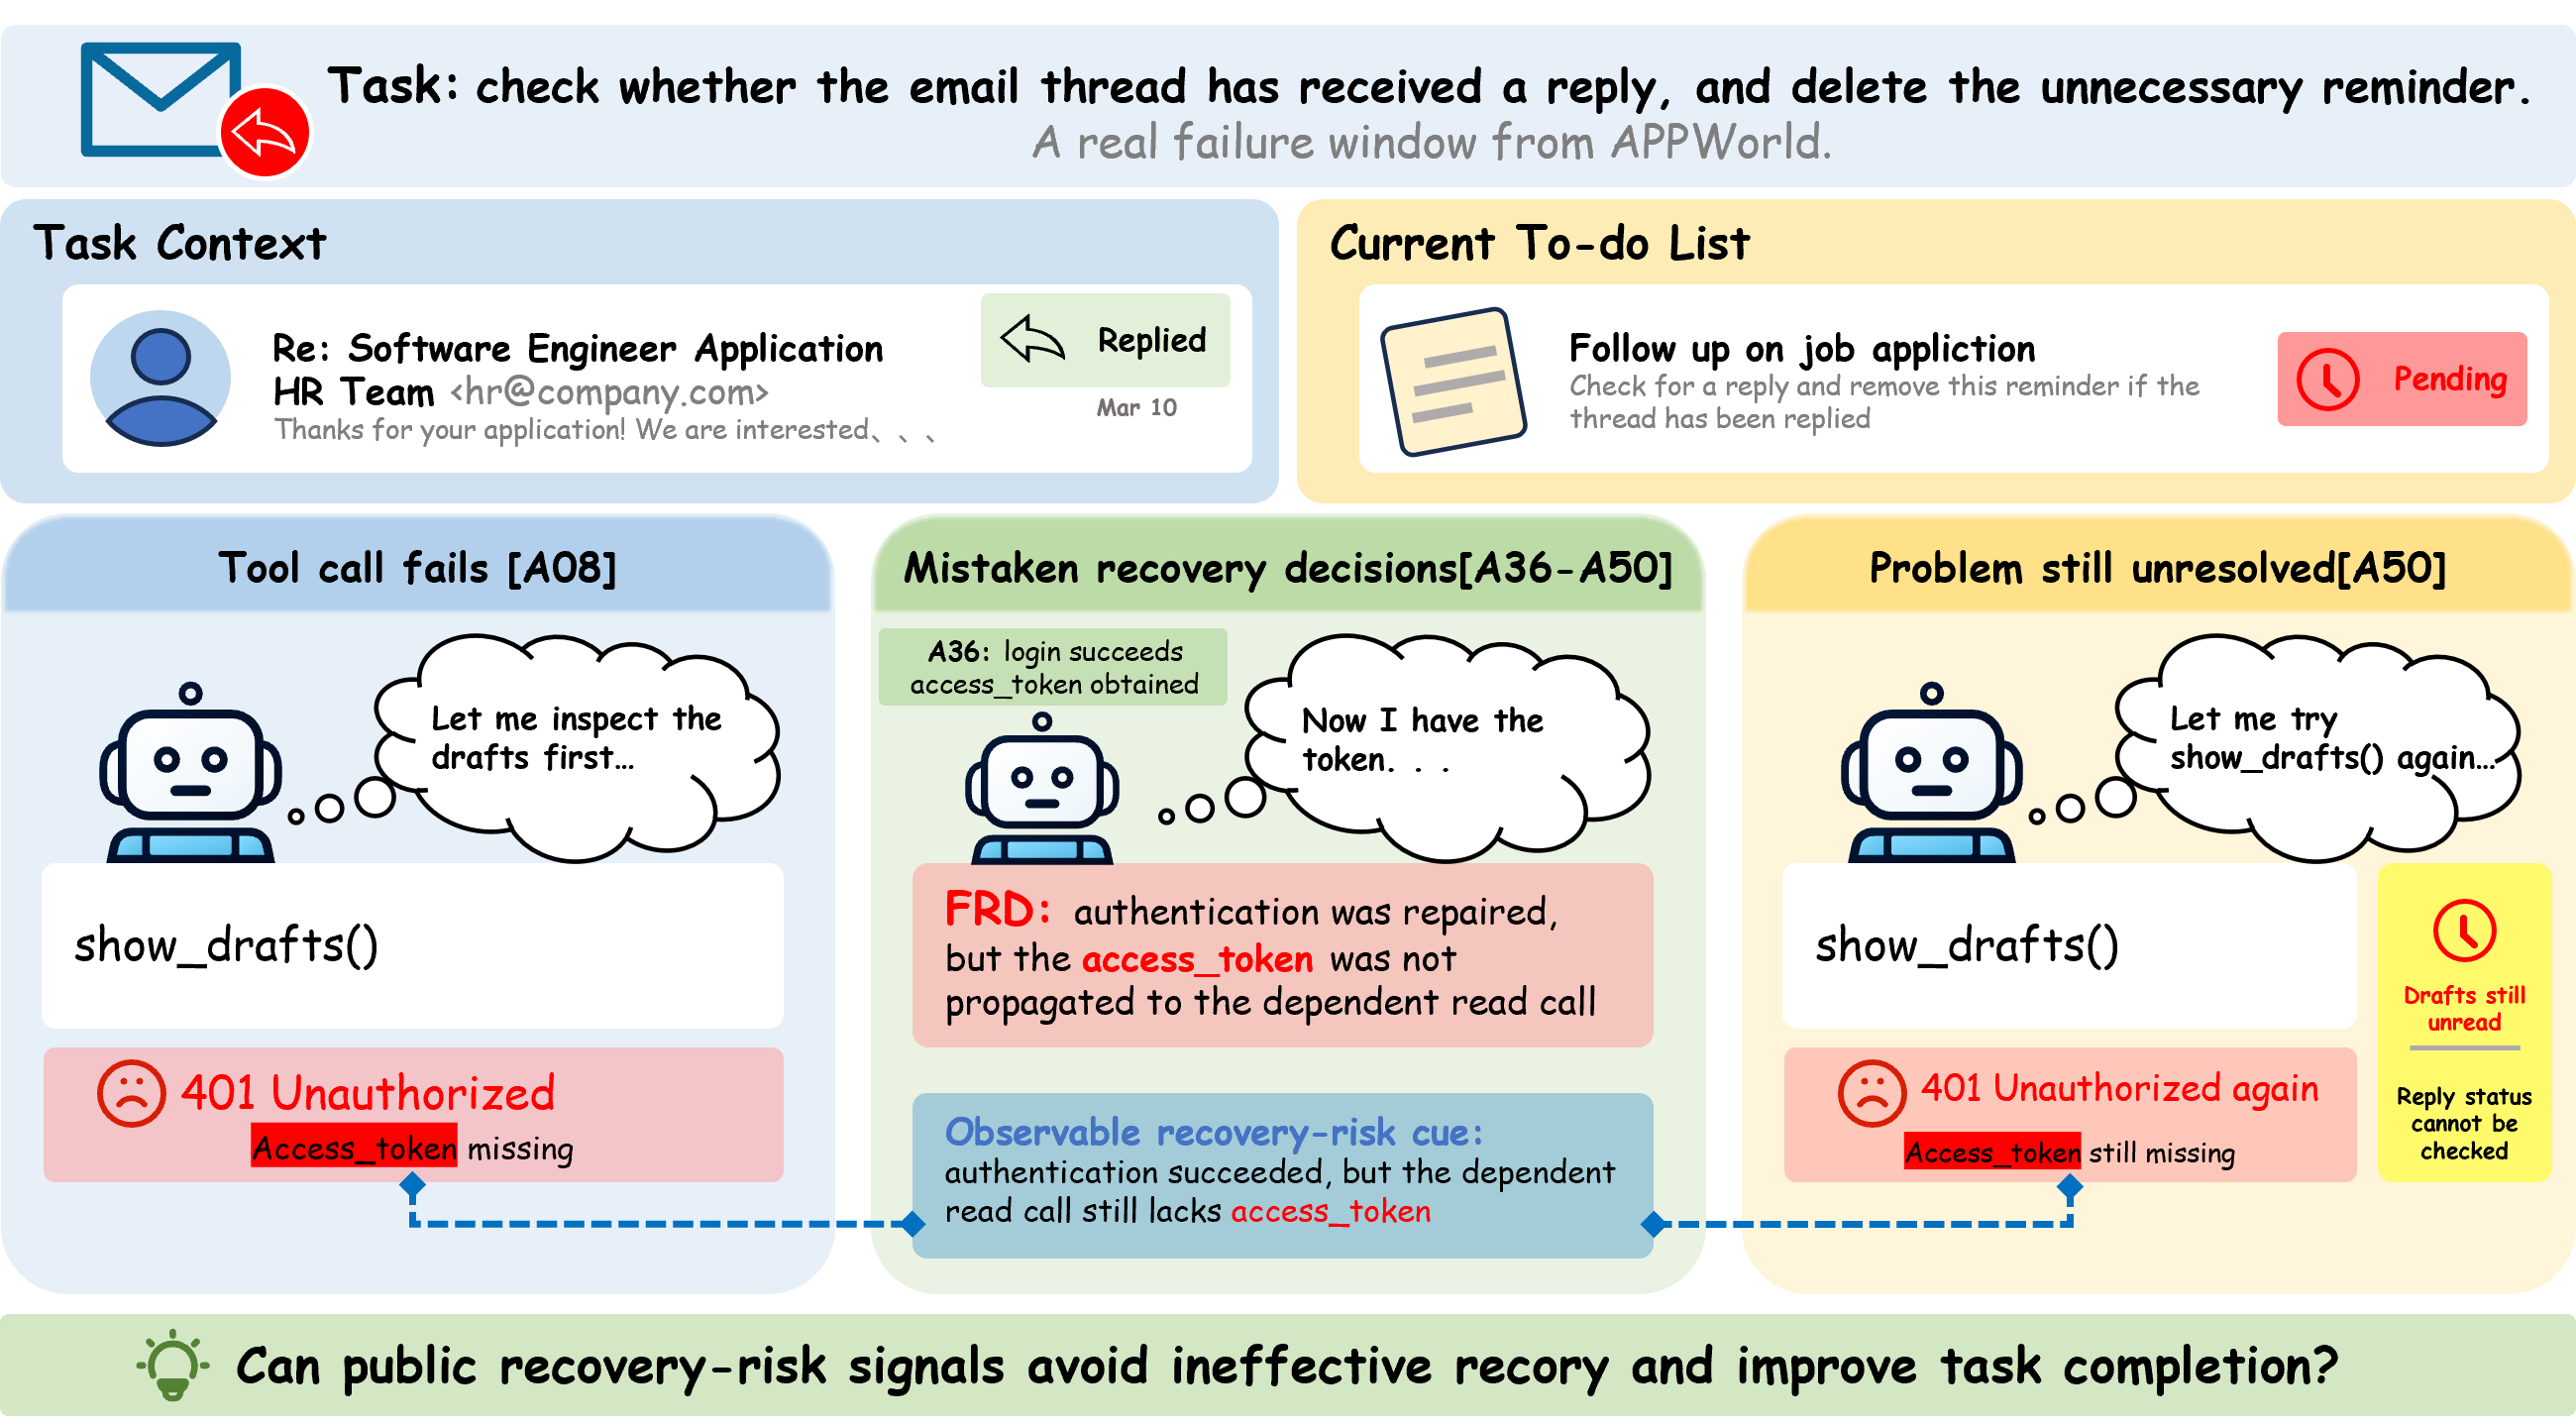
\includegraphics[width=\linewidth]{figures/frd_phenomenon.png}
\caption{Entering recovery does not restore task progress. The model obtains a valid token at A36 but omits it again at A50, reproducing the error from A08.}
\label{fig:frd-phenomenon}
\vspace{-8pt}
\end{wrapfigure}
The difficulty is that repairing an execution is a harder problem than detecting that repair is needed, and the two differ in kind, which matches reported limits of intrinsic self-correction \citep{huang2024selfcorrect,gou2024critic}. Detection is a local judgment about one observation, since an error message or an empty result declares itself. Repair is a constraint satisfaction problem over the whole execution, because the corrective action must name the right target, carry arguments grounded in the current state, respect an order that earlier calls have already fixed, and leave the prerequisites of every later call intact. Figure~\ref{fig:frd-phenomenon} shows a real case from AppWorld. The model calls \api{show\_drafts()} at step A08 without an access token and receives an authentication error. It correctly diagnoses the missing credential and logs in at A36, obtaining a valid token. At A50 it retries the original read and omits the token again, reproducing the identical error. Every individual decision looks reasonable and the recovery action itself returns success, yet the failure lives in the gap between obtaining a prerequisite and applying it to the dependent call. We call this a \emph{Failed Recovery Decision}, which can arise from a wrong target, ungrounded arguments, an invalid action order, a skipped verification, or a premature stop. Therefore, the decisive question is not whether a model notices an error but whether the action it takes in response restores the execution.



What makes this failure mode hard to act on is that it cannot be recognized while the model is still running, and the obstacle is structural instead of practical. Judging a repair means attributing a later outcome to an earlier decision, which is a credit assignment question, and the evidence that settles it consists of consequences that the trajectory has yet to produce. An online controller therefore has no access to the very label it would need in order to correct itself. Existing test-time approaches sidestep the problem instead of solving it. Sampling-based methods generate several complete trajectories and select among the finished candidates \citep{oppo_tts2025,wang2023selfconsistency}, so the comparison happens after all repairs have already been committed. Reflection-based methods feed a verbal critique into a retry \citep{shinn2023reflexion,madaan2023selfrefine}, which reuses free-form text that carries no guarantee about which prior structure may be reused. In essence, both families treat a comparison as a terminal judgment, so the information it produces is discarded instead of being converted into a constraint on the next attempt.



To this end, we propose \method, a test-time scaling framework that turns the evidence of a comparison into a constraint on the execution that follows. \method separates what is adjudicable offline from what is usable online. Failed Recovery Decision is reserved as a retrospective label for analysis, while the \emph{Recovery-risk Disagreement Signal} is extracted from public traces during execution. As illustrated in Figure~\ref{fig:rise-overview}, the signal determines where the next attempt must re-ground itself, an accepted trajectory is retained across rounds so that progress is never lost, and each pairwise comparison is converted into structural credit whose provenance is checked before use. Specifically, to keep guidance transferable across fresh environments, \method abstracts every event into a value-free shape that records operation, tool, field names, and result class while discarding literal arguments, so the next rollout is told which structures to preserve or avoid without being handed reusable identifiers. To extract information from failure itself, \method derives preserve credit only from the selected side and avoid credit only from the rejected side, which makes a rejected candidate an active contributor instead of a discarded sample. Through this combination of directed generation and source-constrained credit, \method learns within a single task which structures a later execution should repeat.

We evaluate \method against Vanilla and Best-of-4 on four tool-calling benchmarks under a matched budget of complete rollouts. Experimental results show that \method outperforms Best-of-4 on every benchmark and every evaluated model, raising AppWorld Test-Challenge scenario completion from 82.73 to 91.37 and OccuBench PASS@1 from 70.68 to 76.96 with GPT-5.6-Sol. Notably, the gains concentrate on scenario-level consistency, where an entire group of related tasks must succeed together. In summary, our key contributions are three-fold.
\begin{itemize}[leftmargin=1em, itemsep=-1ex, topsep=0ex]
    \item \textbf{Problem Formulation}: To the best of our knowledge, we are the first to isolate failed repair as a distinct failure mode in tool-using language models, and to separate its retrospective label from the public evidence that remains usable during execution.
    \item \textbf{Method}: We propose \method, which directs fresh rollouts by public recovery risk, retains an accepted trajectory, and converts bilateral comparison into source-constrained structural credit, so that rejected candidates still shape later attempts.
    \item \textbf{Strong Performance}: Experimental results on four tool-calling benchmarks show that \method surpasses Best-of-4 by up to 8.64 points on scenario goal completion under an identical rollout budget, and more importantly, its margin widens precisely on the metrics that aggregate over correlated tasks.
\end{itemize}

\section{Failed Repair as a Distinct Failure Mode}
\label{sec:analysis}
This section establishes that failed repair is frequent enough to matter and harmful enough to target, and that what distinguishes it from ordinary error is what makes it unusable online. Appendix~\ref{app:adjudication} states the adjudication procedure, and the analyses use DeepSeek-v4.1-Flash.

\textbf{Retrospective Label}\quad To reason about repair without leaking evaluator information into execution, we first fix what can be judged only after the fact. Let $\tau=(a_1,o_1,\ldots,a_T,o_T,r)$ denote a tool-calling trajectory with actions $a_t$, public observations $o_t$, and final response $r$. For an audited recovery episode $w$, let $F_w,D_w,I_w,L_w$ indicate a recovery need, a recovery attempt, an incorrect decision, and an adverse outcome attributable to that decision. A Failed Recovery Decision is
\begin{equation}
\mathrm{FRD}(\tau)=\mathbf{1}\!\left[\exists w\in\mathcal{W}(\tau):F_wD_wI_wL_w=1\right],
\label{eq:frd}
\end{equation}
where $\mathcal{W}(\tau)$ is the set of recovery episodes in $\tau$. A recovery need may begin with a failed call, an inconsistent state, or a user-reported problem, and an adverse outcome includes leaving the target unrecovered or committing a mutation that a known constraint forbids. Equation~\ref{eq:frd} requires an outcome, so it becomes available only once execution completes.

\textbf{Online Signal}\quad To obtain a quantity that a controller may legally consult while running, we drop the outcome requirement. Given task $x$ and the public prefix through action $j$, the Recovery-risk Disagreement Signal is
\begin{equation}
R_{\tau,j}=f_{\mathrm{risk}}(x,\tau_{\leq j}),
\label{eq:rds}
\end{equation}
where $f_{\mathrm{risk}}$ collects failure boundaries, repeated mutations, missing read-back, and explicit tool errors from the public trace. Equation~\ref{eq:rds} reads the public trace alone, so it remains available throughout generation. The signal marks where a later attempt should re-ground itself, while Equation~\ref{eq:frd} supplies the retrospective judgment used for offline analysis.

\textbf{Prevalence and Harm}\quad To establish that failed repair is a recurring phenomenon instead of an artifact of one environment, we measure both quantities under Vanilla and Best-of-4 on the three benchmarks whose traces expose tool-level recovery episodes. As shown in Figure~\ref{fig:frd-rds-distribution}, public recovery risk appears in every benchmark and persists after Best-of-4 selection, while the adjudicated label is uniformly rarer because it additionally demands a complete evidence chain. Trajectories carrying the label complete substantially fewer tasks under either baseline, and the gap is widest where tasks carry the deepest stateful dependencies, since a mis-grounded repair propagates through every dependent call. The persistence after selection is the operative finding, because choosing among four finished trajectories reduces the underlying risk without removing it. Overall, these results motivate using recovery evidence to steer generation itself, and Equation~\ref{eq:rds} is the quantity a generator reads to do so.

\begin{figure}[t]
\centering
\begin{minipage}[t]{0.215\linewidth}\vspace{0pt}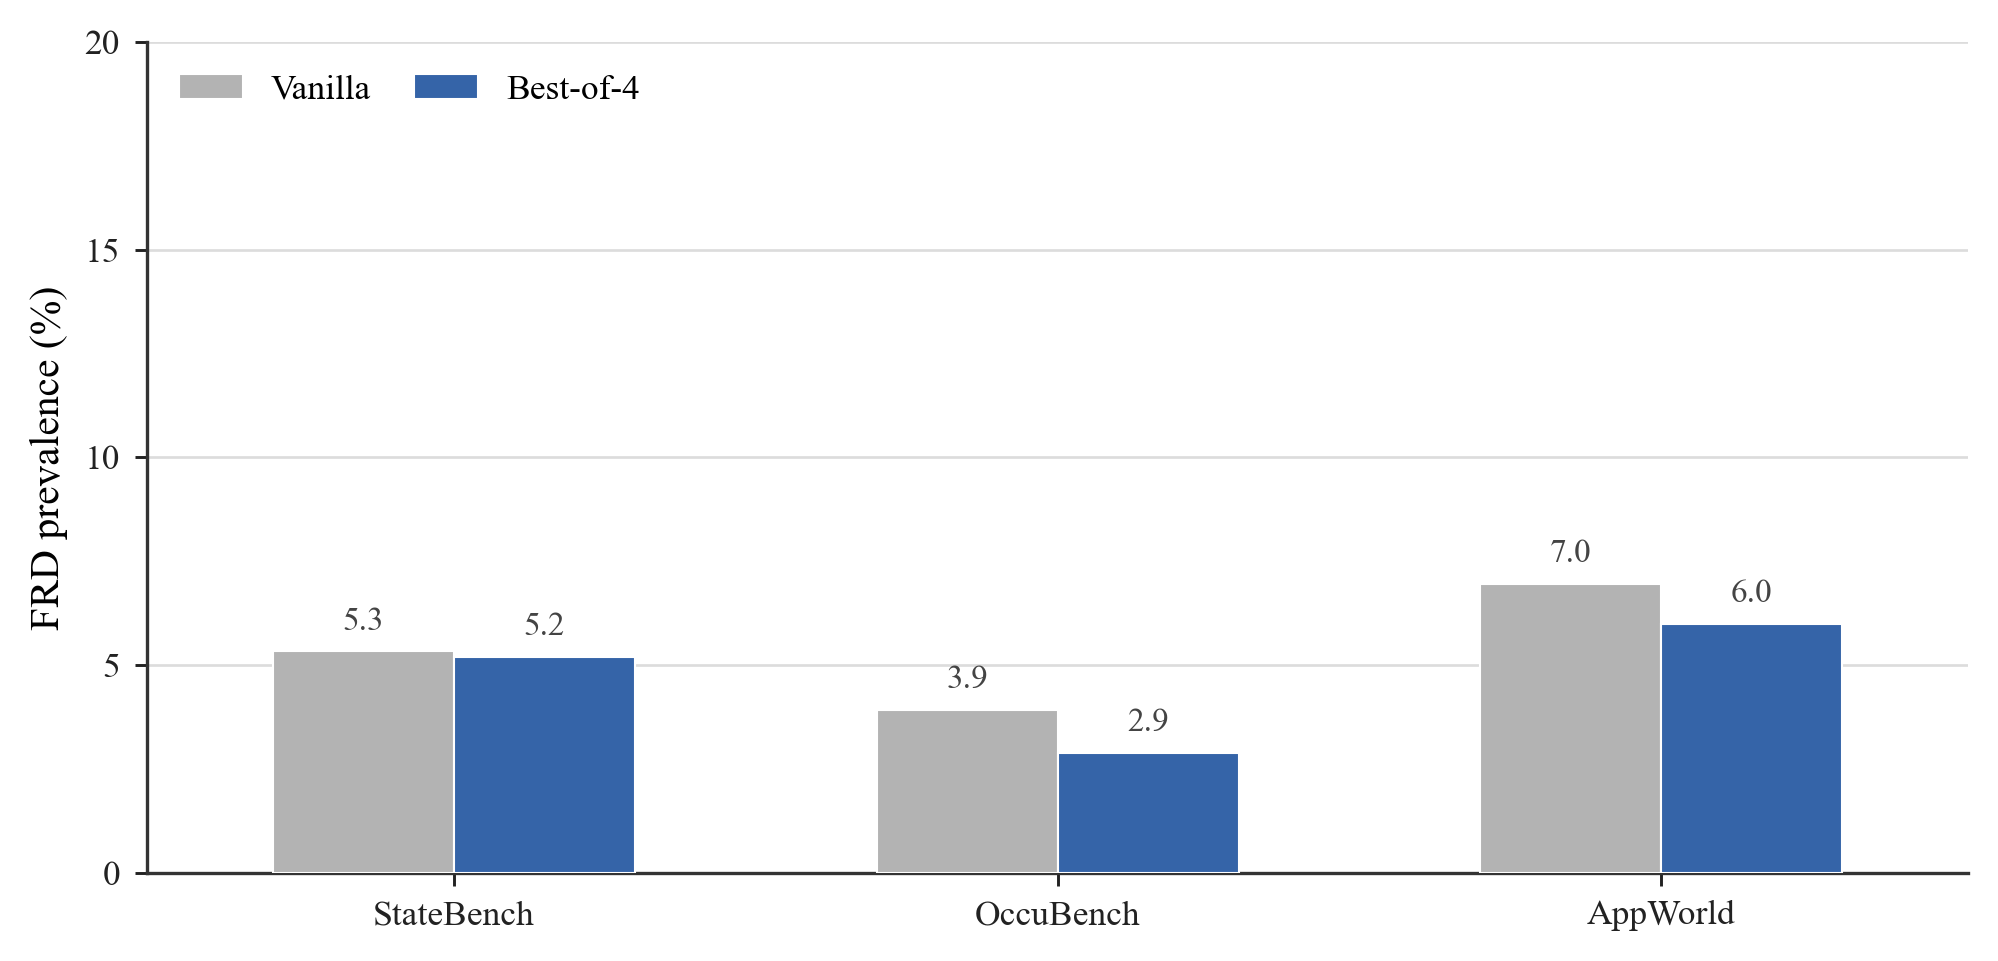
\includegraphics[width=\linewidth]{figures/baseline_frd.png}\par\vspace{2pt}\raggedright\normalfont\scriptsize (a) Failed repair, prevalence.\par\end{minipage}\hfill
\begin{minipage}[t]{0.215\linewidth}\vspace{0pt}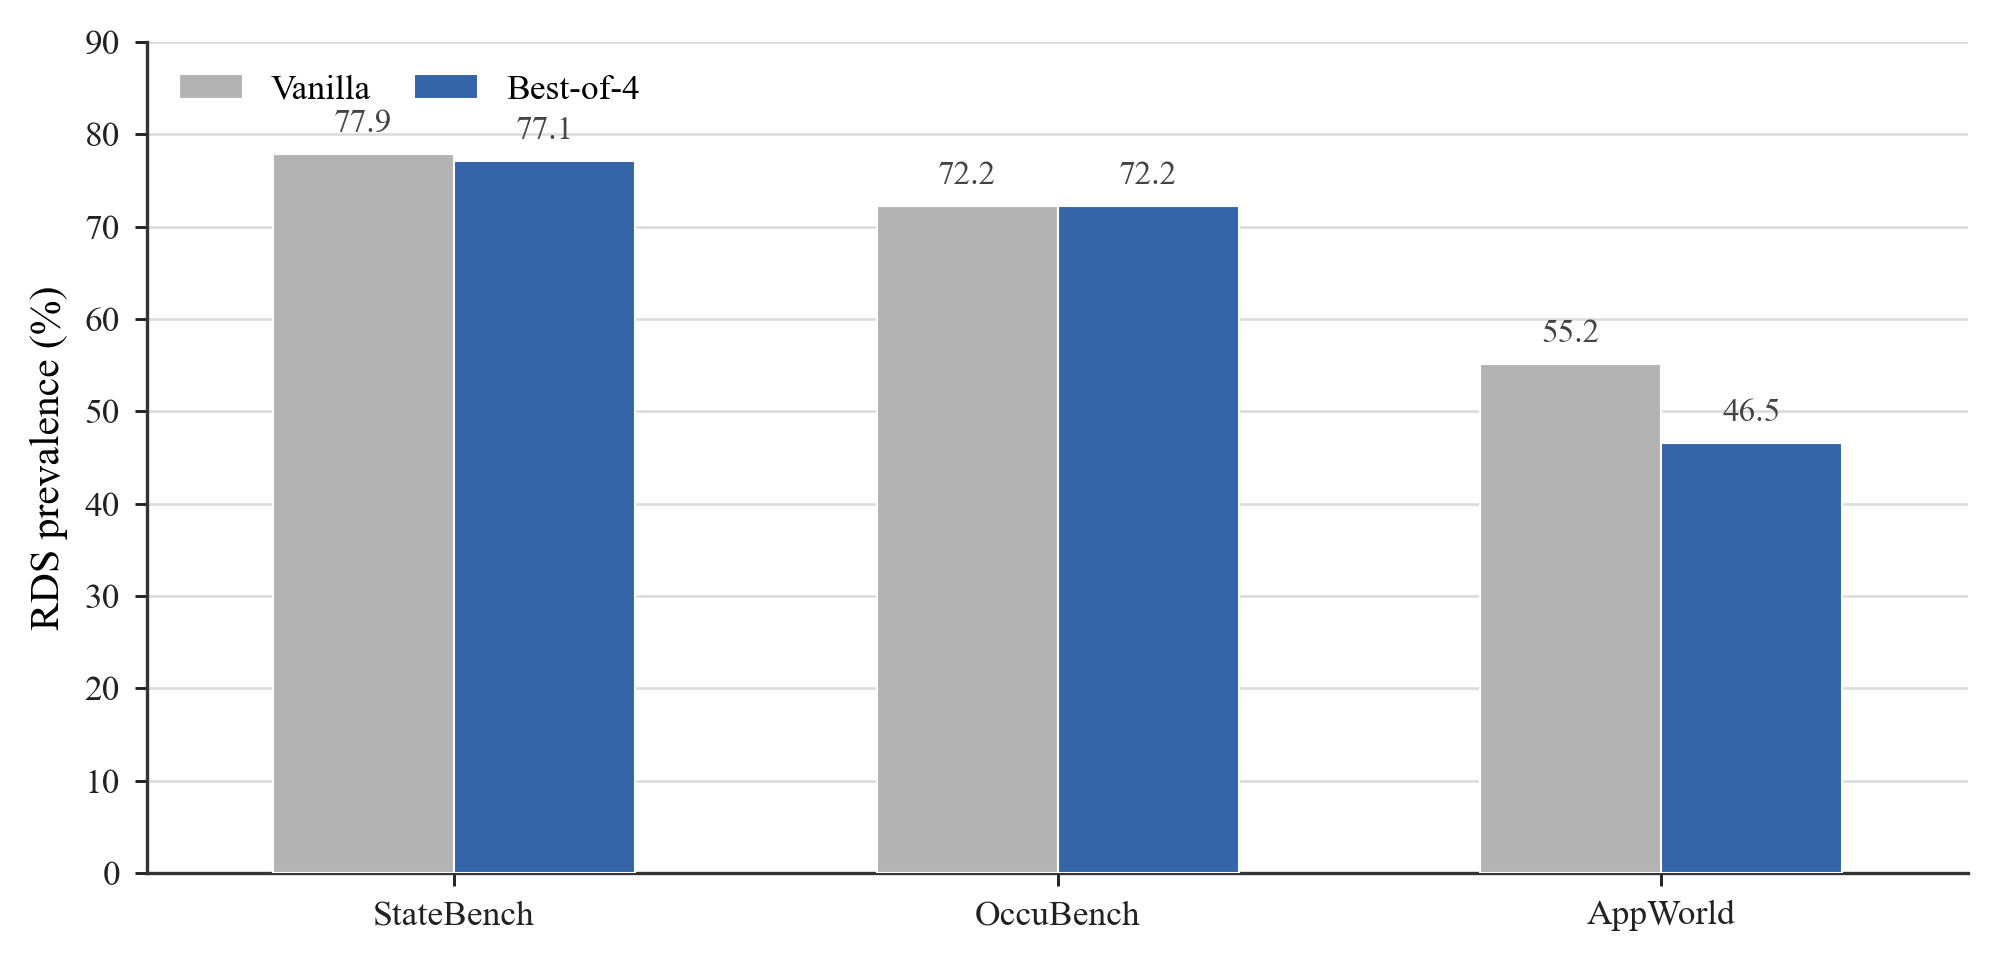
\includegraphics[width=\linewidth]{figures/baseline_rds.png}\par\vspace{2pt}\raggedright\normalfont\scriptsize (b) Recovery risk, prevalence.\par\end{minipage}\hfill
\begin{minipage}[t]{0.215\linewidth}\vspace{0pt}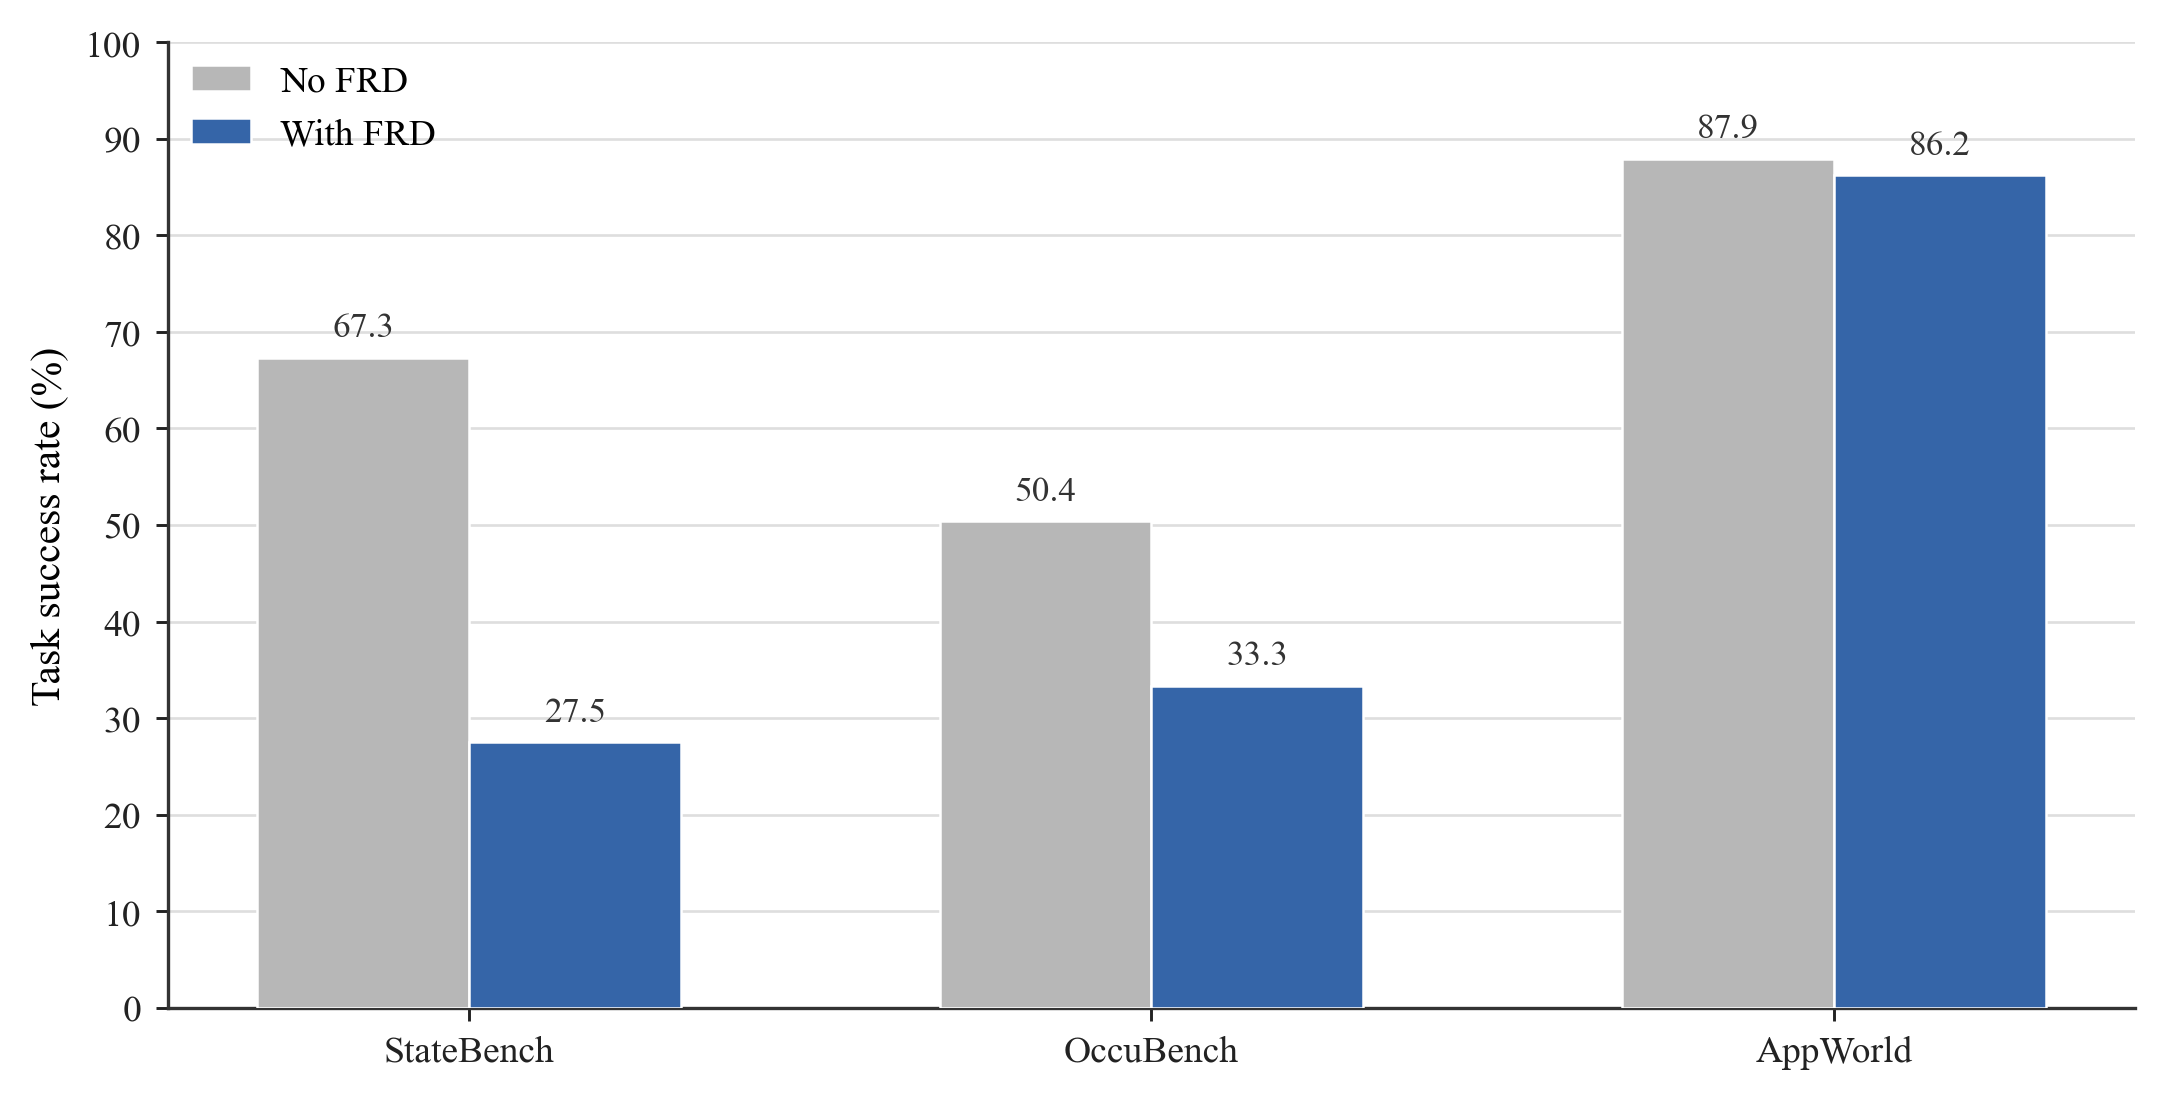
\includegraphics[width=\linewidth]{figures/frd_success_vanilla.png}\par\vspace{2pt}\raggedright\normalfont\scriptsize (c) Task success, Vanilla.\par\end{minipage}\hfill
\begin{minipage}[t]{0.215\linewidth}\vspace{0pt}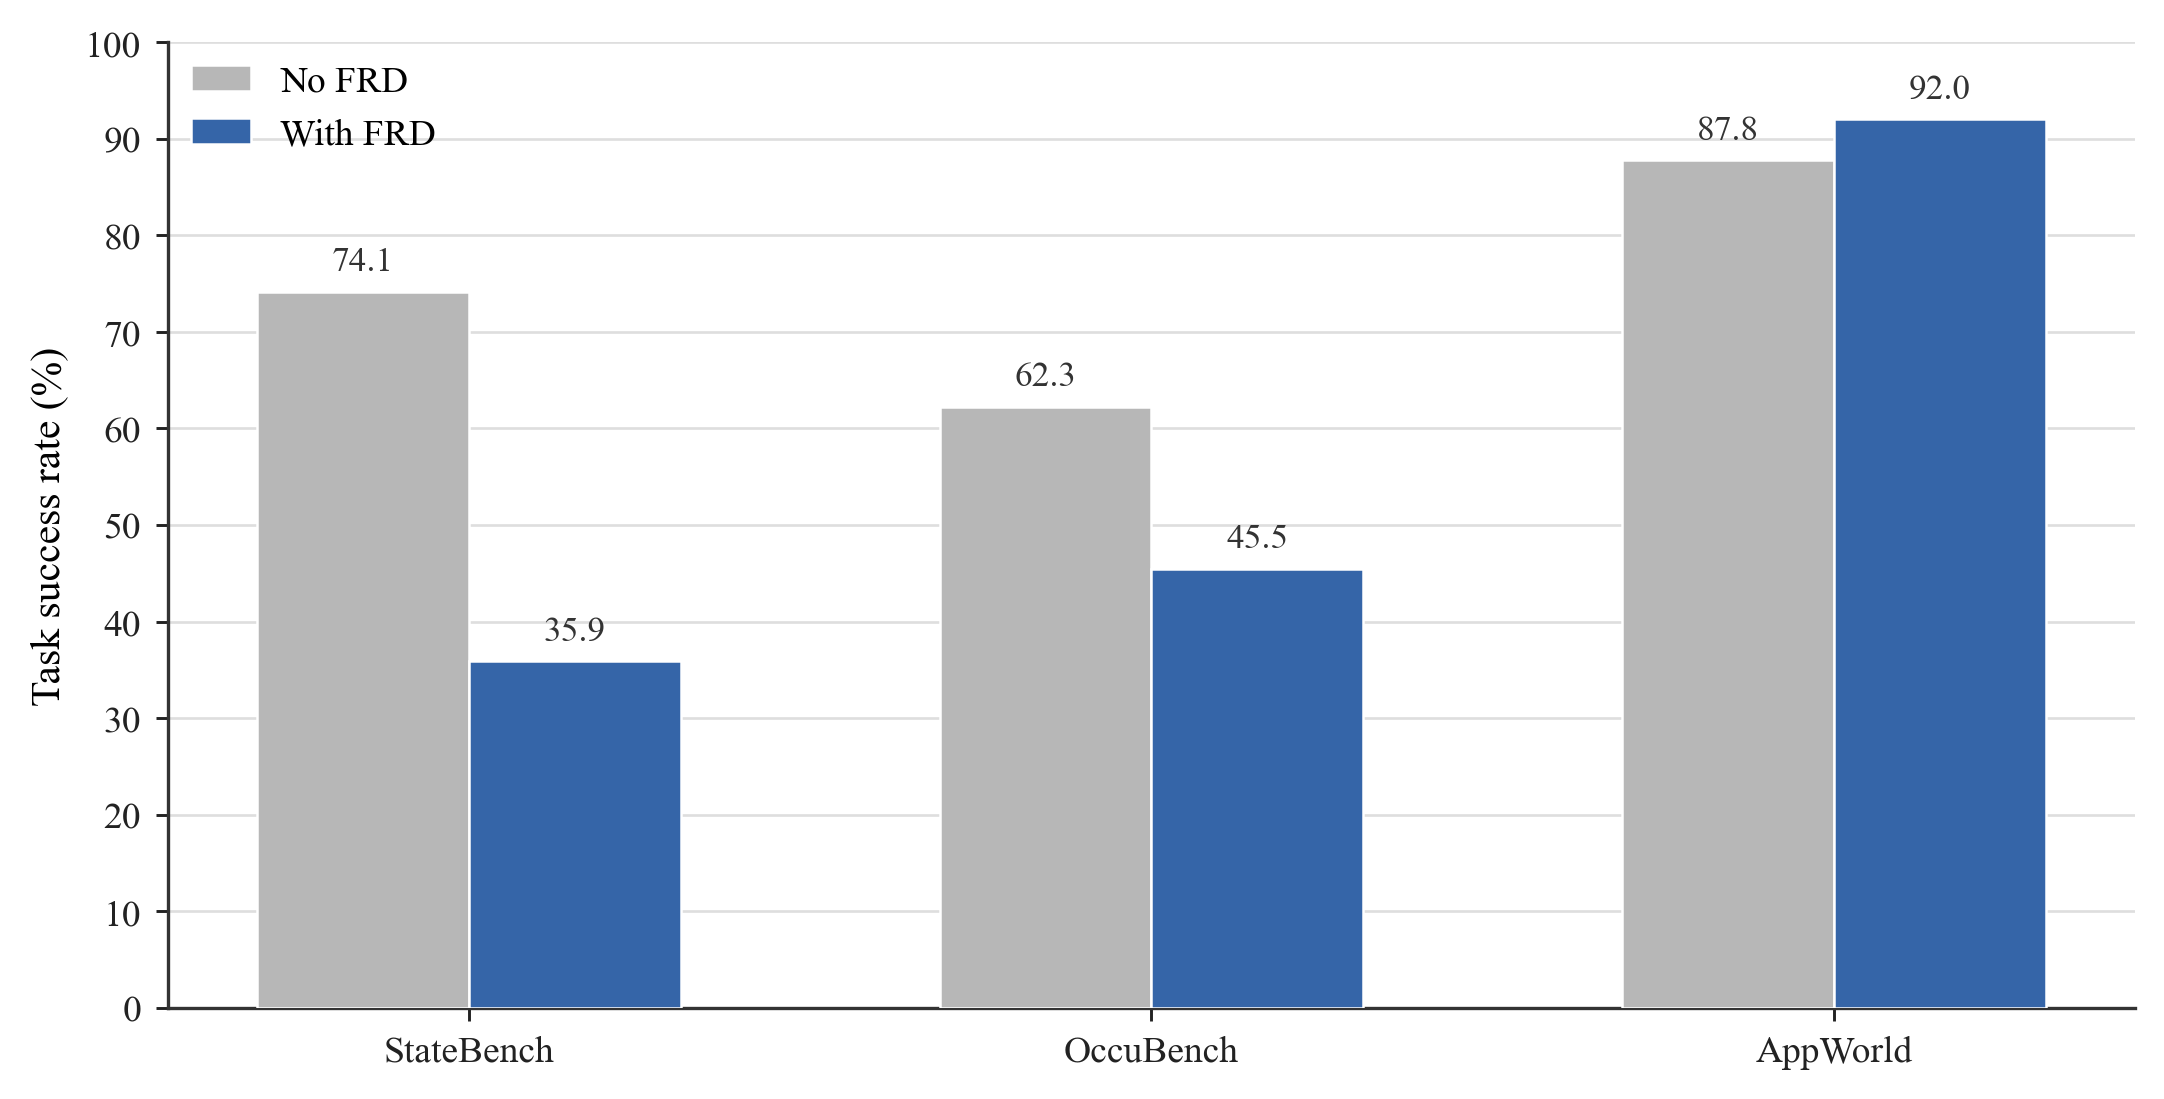
\includegraphics[width=\linewidth]{figures/frd_success_best4.png}\par\vspace{2pt}\raggedright\normalfont\scriptsize (d) Task success, Best-of-4.\par\end{minipage}
\caption{Failed repair is common and harmful. Both the adjudicated label and the public signal persist after Best-of-4 selection (a, b), and trajectories carrying the label complete substantially fewer tasks under either baseline (c, d), with the widest gap where tasks carry the deepest stateful dependencies.}
\label{fig:frd-rds-distribution}
\end{figure}

\section{RISE}
\label{sec:rise}
\begin{figure}[t]
\centering
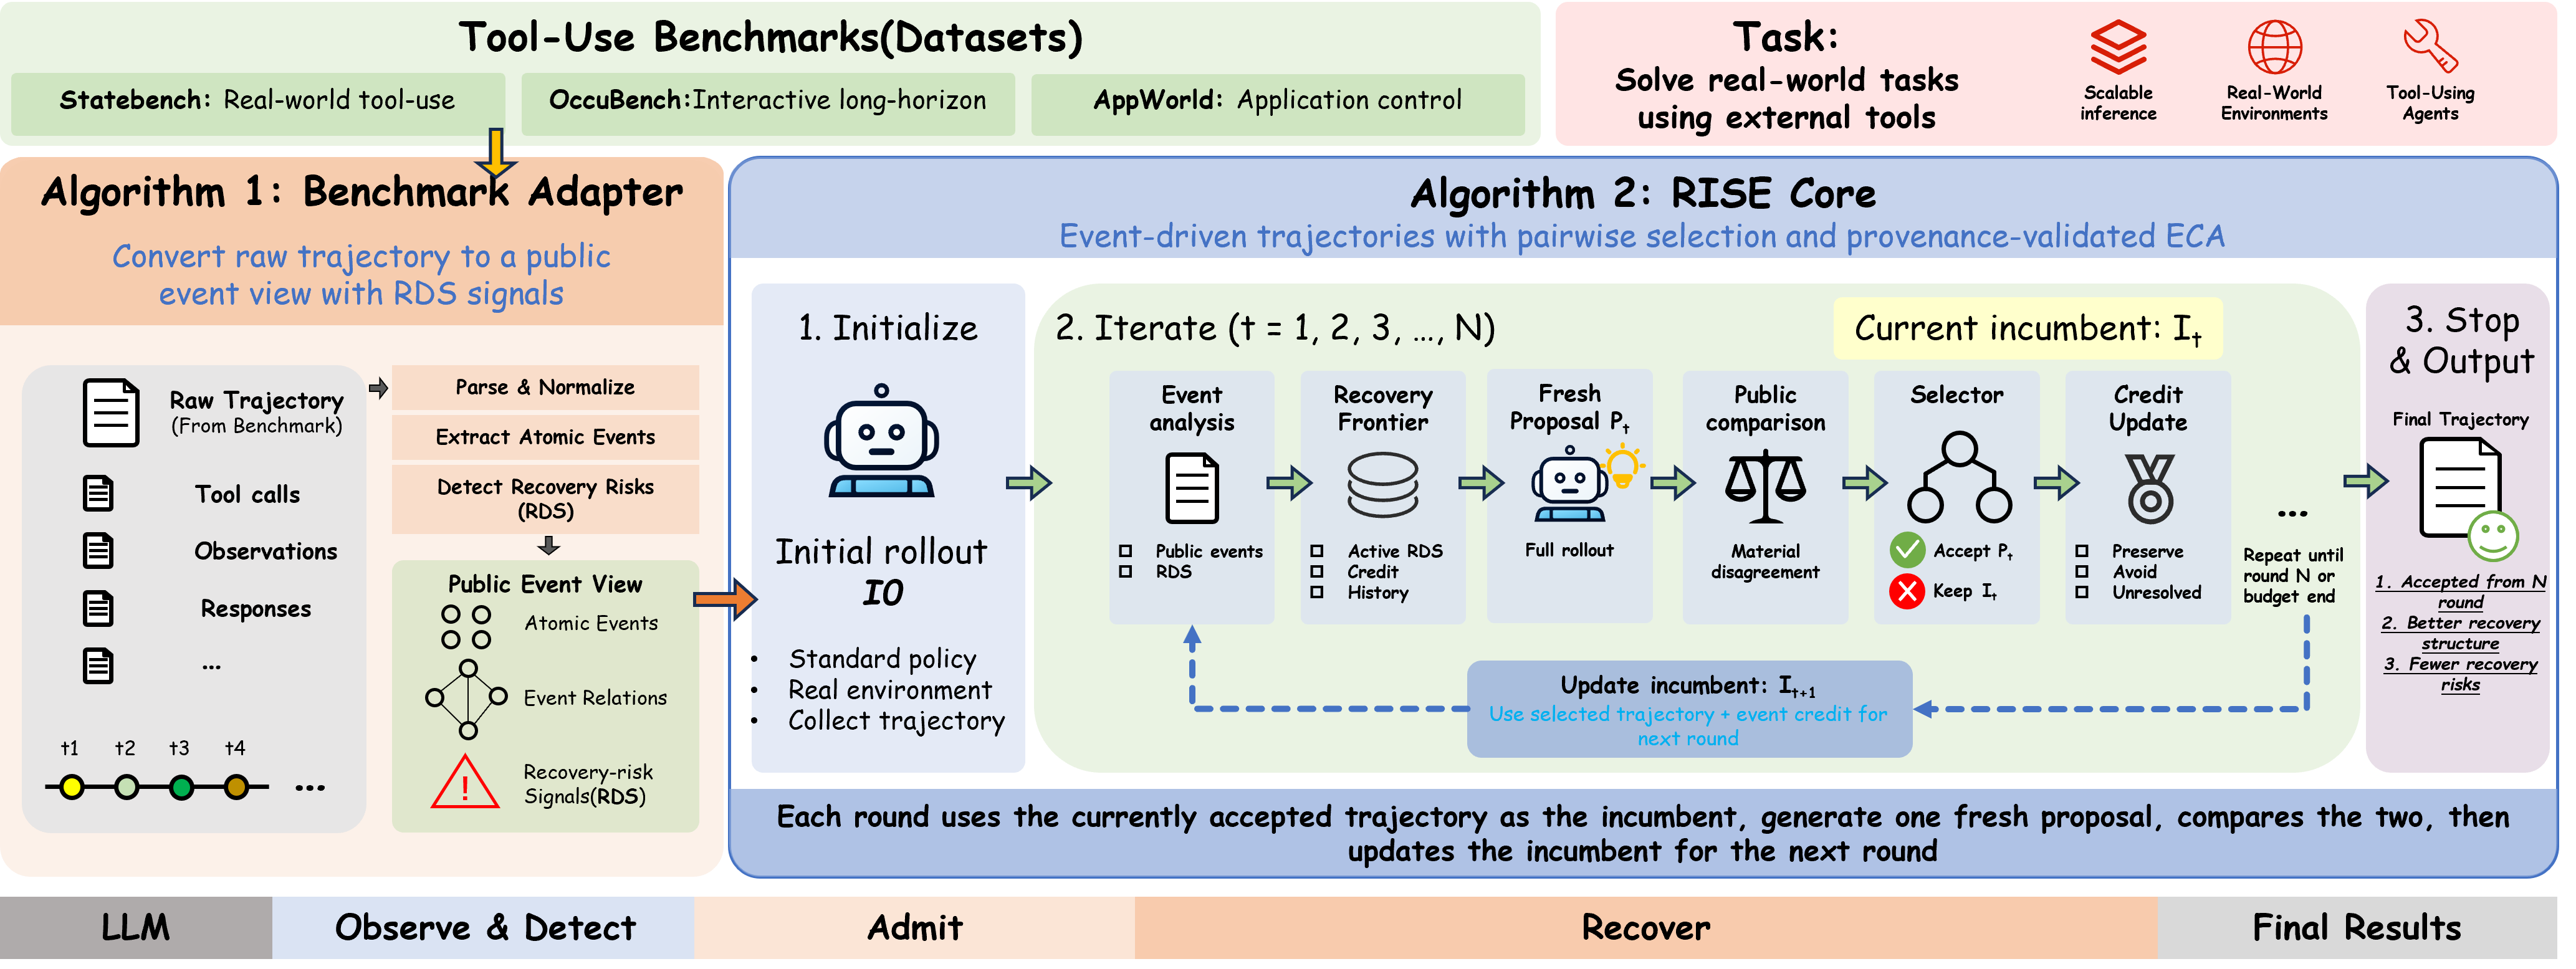
\includegraphics[width=0.74\linewidth]{figures/rise_method_overview.png}
\caption{\method turns each comparison into guidance for the next attempt. Public interactions are mapped to events and recovery risk, a frontier directs one fresh complete rollout, and bilateral credit from both the selected and the rejected candidate constrains later rounds.}
\label{fig:rise-overview}
\end{figure}
Section~\ref{sec:analysis} establishes that repair quality is both consequential and unverifiable online. \method addresses this by organizing three updates into a single search over complete executions. The complete trajectory is the unit of generation and acceptance, the public event is the unit of analysis and feedback, and a fresh environment is the boundary of every execution.

\subsection{Accepted Trajectory as the Search State}
To ensure that guidance never destroys progress already achieved, \method maintains an accepted trajectory instead of continuously editing one attempt. The search begins from an unguided rollout with empty credit and history, and each round executes the original task in a fresh environment, so cross-round guidance may carry event structure while every execution grounds its own identifiers and values.

\subsection{Recovery Frontier for Directed Rollouts}
To convert public risk into an actionable instruction, \method compiles the current trajectory into an event view and builds a frontier that names what the next attempt must recheck. The event map produces $V_t=f_{\mathrm{event}}(I_t)=(E_t,G_t,R_t)$, where $E_t$ contains atomic events with operation, argument, and result fields, $G_t$ contains supported transaction groups, and $R_t$ contains public recovery risk. The frontier and the resulting proposal are
\begin{equation}
\mathcal{F}_t=f_{\mathrm{front}}(V_t,C_t,H_t),\qquad
P_t=f_{\mathrm{roll}}(x,\mathcal{F}_t),
\label{eq:frontier}
\end{equation}
where $f_{\mathrm{front}}$ fuses current risk with accumulated credit and permitted history, and $f_{\mathrm{roll}}$ executes one complete rollout in a fresh environment. Current risk sets the active focus, and an unresolved issue from earlier credit fills that role when no current risk is present. The frontier is a guidance package for a new execution, never a set of partially executed states.

\subsection{Material Disagreement as a Selection Gate}
To avoid spending a comparison on two trajectories that differ only cosmetically, \method first tests whether the candidates disagree in a way that matters. The gate computes $D_t=f_{\mathrm{cmp}}(f_{\mathrm{event}}(I_t),f_{\mathrm{event}}(P_t))$ over transaction content and ordering. When $D_t=0$, the accepted trajectory is retained and no selection is invoked. Otherwise a selector compares the two complete candidates through their public representations and returns $q_t\in\{\mathrm{inc},\mathrm{prop}\}$, giving
\begin{equation}
I_{t+1}=\begin{cases}P_t,&D_t=1\ \text{and}\ q_t=\mathrm{prop},\\[2pt]
I_t,&\text{otherwise},\end{cases}
\label{eq:incumbent}
\end{equation}
where the selector weighs task coverage, grounding, action order, public effects, recovery, verification, and stopping.

\subsection{Bilateral Credit with Source Constraints}
To extract information from the candidate that was rejected, \method derives guidance from both sides of a valid comparison under a provenance rule. Let $V_t^s$ and $V_t^r$ denote the selected and rejected event views. The update is
\begin{equation}
C_{t+1}=f_{\mathrm{credit}}(V_t^s,V_t^r,D_t,q_t,C_t)=(C^{+}_{t+1},C^{-}_{t+1},z_{t+1}),
\label{eq:credit}
\end{equation}
where $C^{+}$ holds structures to preserve, $C^{-}$ holds structures to avoid, and $z$ records an unresolved issue. Preserve credit comes only from the selected side and avoid credit only from the rejected side, and provenance is validated before any structure is written. Every retained structure is then projected into a value-free shape that keeps operation, event class, tool, field names, argument keys, result class, and interaction type while discarding literal values. The projection separates two kinds of knowledge that a comparison produces together. Structural knowledge, such as the requirement that a read of this resource carry an authenticated session, holds in any instance of the task, while instance knowledge, such as the token string obtained in one episode, holds only in the environment that produced it. Carrying the first across rounds is what makes guidance useful, and discarding the second is what keeps it correct.

This construction yields a property that selection-only scaling cannot express. Since eligibility for preserve credit depends on whether a structure also appears on the rejected side, exchanging the rejected candidate changes the guidance even when the accepted trajectory is unchanged. A comparison therefore returns both a decision about which trajectory to keep and a constraint on how the next attempt is generated, and the second survives even when the first changes nothing. The accepted trajectory, updated credit, and permitted history then pass into the next frontier, and the search returns the accepted trajectory when the schedule ends, so a schedule of $N$ proposals consumes $N+1$ complete rollouts. Algorithm~\ref{alg:rise} in Appendix~\ref{app:implementation} summarizes the procedure.

\section{Experiments}

\subsection{Benchmarks}
We evaluate on four benchmarks that cover representative forms of complex tool calling, namely StateBench for stateful conversational tool use, AppWorld \citep{trivedi2024appworld} for persistent cross-application interaction, OccuBench for professional tool use, and DeepPlanning Travel for constrained planning. Task counts, splits, and metric definitions appear in Appendix~\ref{app:benchmarks}.

\subsection{Setup}
We compare \method with Vanilla, which executes a single rollout, and with Best-of-$N$, which we adopt as the representative test-time scaling method because sampling, verification, and result merging have been most systematically studied in that setting for tool-using agents \citep{oagents2025,oppo_tts2025}. We set $N=4$ following its released configuration, and we cap \method at the same number of complete rollouts, so the four candidates of the baseline correspond to one initial trajectory followed by three guided proposals. This makes $4$ the shared upper bound on both the sampling width of the baseline and the iteration depth of \method. We evaluate DeepSeek-v4.1-Flash, Qwen3.8-Max, and GPT-5.6-Sol on all four benchmarks. Tasks, tools, simulators, and evaluators are held fixed across methods within each cohort, and every online decision reads the public trace.

\subsection{Main Results}
To determine whether directed rollouts outperform independent sampling at equal cost, we compare all three settings under an identical budget of complete rollouts. As shown in Tables~\ref{tab:statebench}--\ref{tab:deepplanning}, \method improves over both baselines across all four benchmarks and all evaluated models, raising OccuBench PASS@1 from 68.85 to 74.35 with Qwen3.8-Max and AppWorld Test-Challenge scenario completion from 82.73 to 91.37 with GPT-5.6-Sol. Best-of-4 already captures most of what independent sampling offers, lifting OccuBench PASS@1 from 57.85 to 68.85, and \method adds a further 5.50 points at the same rollout budget, which sample diversity cannot explain because the number of complete executions is identical. More importantly, unlike independent sampling, \method constrains where each new rollout spends its attempt and carries the outcome of each comparison forward, so later rollouts are directed instead of independent draws.

The margin over Best-of-4 varies with a property of the failure distribution, and reading it this way explains an otherwise puzzling result. Independent sampling protects against \emph{stochastic} failure, where four draws rarely go wrong in the same place, so the maximum over the pool improves as the pool grows. It offers no protection against \emph{systematic} failure, where a model omits the same prerequisite in every draw, because enlarging a pool of identically biased samples leaves the maximum unchanged. For instance, on AppWorld Test-Normal with DeepSeek-v4.1-Flash, Best-of-4 leaves task completion unchanged at 91.07, so its failures there are the repeatable kind, and this is precisely where \method gains, lifting the same metric to 92.26, since an avoided structure recorded from one rejected candidate is unavailable to every later attempt.

This reading also predicts which metric should move first. Scenario goal completion requires every task in a related group to pass, so a defect that recurs across the group costs the entire score while task-level completion loses only the affected members. A metric that aggregates over correlated tasks is therefore more sensitive to systematic failure than to stochastic failure. On AppWorld Test-Challenge, \method improves scenario completion over Best-of-4 by 4.31, 7.20, and 8.64 points across the three models, against 1.68, 4.31, and 4.55 points for task completion on the same split, and the ordering holds for every evaluated model, which is the behavior the mechanism predicts instead of an incidental property of one benchmark. Overall, \method's strong results under a matched budget highlight its advantage in converting evidence about repeatable failure into a constraint, which is information that no amount of independent sampling can supply.

\begin{table}[t]
\centering
\small
\begin{minipage}[t]{0.63\linewidth}
\centering
\caption{Results on StateBench. PASS$^5$ requires completion in all five independent runs. UX is rated from 1 to 5. \textbf{Bold} marks the best within each model.}
\label{tab:statebench}
\setlength{\tabcolsep}{4pt}
\begin{tabular}{llccc}
\toprule
Method & Base LLM & PASS@1 & PASS$^5$ & UX \\
\midrule
Vanilla & DeepSeek-v4.1-Flash & 65.20 & 38.67 & 3.9709 \\
Best-of-4 & DeepSeek-v4.1-Flash & 72.13 & 46.67 & 4.1428 \\
\textbf{\method} & DeepSeek-v4.1-Flash & \textbf{72.67} & \textbf{48.67} & \textbf{4.1499} \\
\midrule
Vanilla & Qwen3.8-Max & 69.33 & 41.33 & 4.0217 \\
Best-of-4 & Qwen3.8-Max & 76.00 & 49.33 & 4.1893 \\
\textbf{\method} & Qwen3.8-Max & \textbf{81.33} & \textbf{54.67} & \textbf{4.3512} \\
\midrule
Vanilla & GPT-5.6-Sol & 71.33 & 42.00 & 4.0658 \\
Best-of-4 & GPT-5.6-Sol & 78.00 & 50.67 & 4.2374 \\
\textbf{\method} & GPT-5.6-Sol & \textbf{82.67} & \textbf{56.67} & \textbf{4.3981} \\
\bottomrule
\end{tabular}
\end{minipage}\hfill
\begin{minipage}[t]{0.35\linewidth}
\centering
\caption{Results on OccuBench. PASS@1 is the average completion rate over the evaluation instances. `DeepSeek', `Qwen' and `GPT' are DeepSeek-v4.1-Flash, Qwen3.8-Max and GPT-5.6-Sol. \textbf{Bold} marks the best within each model.}
\label{tab:occubench}
\setlength{\tabcolsep}{4pt}
\begin{tabular}{llc}
\toprule
Method & Base LLM & PASS@1 \\
\midrule
Vanilla & DeepSeek & 49.74 \\
Best-of-4 & DeepSeek & 61.78 \\
\textbf{\method} & DeepSeek & \textbf{63.35} \\
\midrule
Vanilla & Qwen & 57.85 \\
Best-of-4 & Qwen & 68.85 \\
\textbf{\method} & Qwen & \textbf{74.35} \\
\midrule
Vanilla & GPT & 59.69 \\
Best-of-4 & GPT & 70.68 \\
\textbf{\method} & GPT & \textbf{76.96} \\
\bottomrule
\end{tabular}
\end{minipage}
\end{table}

\begin{table}[t]
\centering
\small
\caption{Results on AppWorld. `TGC' is task goal completion and `SGC' is scenario goal completion, which requires every task in a scenario to pass. \textbf{Bold} marks the best within each model.}
\label{tab:appworld}
\begin{tabular}{llcccc}
\toprule
\multirow{2}{*}{Method} & \multirow{2}{*}{Base LLM} & \multicolumn{2}{c}{Test-Normal} & \multicolumn{2}{c}{Test-Challenge} \\
\cmidrule(lr){3-4}\cmidrule(l){5-6}
 & & TGC & SGC & TGC & SGC \\
\midrule
Vanilla & DeepSeek-v4.1-Flash & 91.07 & 80.36 & 87.77 & 75.54 \\
Best-of-4 & DeepSeek-v4.1-Flash & 91.07 & 82.14 & 88.01 & 77.70 \\
\textbf{\method} & DeepSeek-v4.1-Flash & \textbf{92.26} & \textbf{85.71} & \textbf{89.69} & \textbf{82.01} \\
\midrule
Vanilla & Qwen3.8-Max & 91.07 & 82.14 & 89.93 & 79.14 \\
Best-of-4 & Qwen3.8-Max & 92.26 & 83.93 & 90.41 & 81.29 \\
\textbf{\method} & Qwen3.8-Max & \textbf{97.02} & \textbf{89.29} & \textbf{94.72} & \textbf{88.49} \\
\midrule
Vanilla & GPT-5.6-Sol & 92.26 & 83.93 & 90.65 & 80.58 \\
Best-of-4 & GPT-5.6-Sol & 93.45 & 85.71 & 91.13 & 82.73 \\
\textbf{\method} & GPT-5.6-Sol & \textbf{97.62} & \textbf{92.86} & \textbf{95.68} & \textbf{91.37} \\
\bottomrule
\end{tabular}
\end{table}



\begin{table}[t]
\centering
\small
\setlength{\tabcolsep}{4pt}
\caption{Results on DeepPlanning Travel. `Deliv.' is plan delivery, `Comm.' and `Pers.' are constraint satisfaction, and `Comp.' is overall planning quality. \textbf{Bold} marks the best within each model and language.}
\label{tab:deepplanning}
\begin{tabular}{llcccccccc}
\toprule
\multirow{2}{*}{Method} & \multirow{2}{*}{Base LLM} & \multicolumn{4}{c}{Chinese} & \multicolumn{4}{c}{English} \\
\cmidrule(lr){3-6}\cmidrule(l){7-10}
 & & Deliv. & Comm. & Pers. & Comp. & Deliv. & Comm. & Pers. & Comp. \\
\midrule
Vanilla & DeepSeek-v4.1-Flash & 85.83 & 39.27 & 27.94 & 32.71 & 90.83 & 45.62 & 25.83 & 35.84 \\
Best-of-4 & DeepSeek-v4.1-Flash & 89.17 & 43.18 & 30.86 & 36.42 & 93.33 & 49.37 & 28.94 & 39.58 \\
\textbf{\method} & DeepSeek-v4.1-Flash & \textbf{95.00} & \textbf{49.86} & \textbf{36.41} & \textbf{42.18} & \textbf{97.50} & \textbf{56.13} & \textbf{34.28} & \textbf{45.31} \\
\midrule
Vanilla & Qwen3.8-Max & 89.17 & 41.63 & 29.73 & 34.58 & 94.17 & 47.86 & 27.64 & 37.79 \\
Best-of-4 & Qwen3.8-Max & 92.50 & 45.82 & 32.85 & 38.47 & 95.83 & 51.74 & 30.92 & 41.63 \\
\textbf{\method} & Qwen3.8-Max & \textbf{95.83} & \textbf{51.47} & \textbf{38.64} & \textbf{44.08} & \textbf{97.50} & \textbf{58.08} & \textbf{36.18} & \textbf{47.18} \\
\midrule
Vanilla & GPT-5.6-Sol & 90.83 & 42.75 & 30.58 & 35.66 & 95.00 & 48.71 & 28.37 & 38.62 \\
Best-of-4 & GPT-5.6-Sol & 93.33 & 46.91 & 33.72 & 39.58 & 96.67 & 52.63 & 31.59 & 42.51 \\
\textbf{\method} & GPT-5.6-Sol & \textbf{98.33} & \textbf{53.36} & \textbf{39.46} & \textbf{45.91} & \textbf{99.17} & \textbf{59.41} & \textbf{37.73} & \textbf{48.69} \\
\bottomrule
\end{tabular}
\end{table}

\section{Analysis}
We conduct the analyses on DeepSeek-v4.1-Flash over the benchmarks that expose tool-level recovery episodes, matching the setting of Section~\ref{sec:analysis}. We first isolate which component of \method carries the gain, then trace the mechanism in a concrete execution, then measure whether the targeted failure mode declines, and finally locate where the improvements fall.

\subsection{Ablation Study on Guidance Components}
\begin{wraptable}{r}{0.40\linewidth}
\vspace{-14pt}
\centering
\small
\caption{Ablation on OccuBench. Each variant removes one guidance component under a fixed rollout budget. \textbf{Bold} marks the best result.}
\label{tab:ablation}
\setlength{\tabcolsep}{5pt}
\begin{tabular}{lc}
\toprule
Method & PASS@1 \\
\midrule
Vanilla & 49.74 \\
Best-of-4 & 61.78 \\
\midrule
No recovery focus & 53.14 \\
No event credit & 57.07 \\
Pairwise summary & 60.73 \\
\midrule
\textbf{\method} & \textbf{63.35} \\
\bottomrule
\end{tabular}
\vspace{-12pt}
\end{wraptable}
To determine whether the three updates in \method contribute independently or function as one coupled process, we remove each in turn on OccuBench while holding the task manifest, model, selector budget, and evaluation protocol fixed. \textbf{No recovery focus} withholds the explicit target supplied by current public risk while retaining events and other feedback. \textbf{No event credit} keeps candidate comparison and acceptance but blocks credit from reaching later rollouts. \textbf{Pairwise summary} replaces structural credit with a free-form summary of the two candidates.

As shown in Table~\ref{tab:ablation}, every variant falls below full \method, and the ordering among them is informative. Withholding the recovery focus produces the steepest decline, at 10.21 points below full \method, which indicates that naming a concrete target contributes more than exposing the raw trajectory, since the trajectory remains fully available in this condition. Blocking event credit costs 6.28 points even though selection and acceptance are untouched. Carrying comparison evidence across rounds is therefore a separate mechanism from choosing a winner. Replacing structural credit with a free-form summary recovers part of that loss and still ends 2.62 points short, which shows that the organization of feedback matters beyond its presence. In particular, each variant also falls below Best-of-4 at the same rollout budget, which locates \method within a general trade. Independent sampling spends its budget on variance, while directed search spends it on information, committing later attempts to what earlier ones revealed. A method that commits to direction without an accurate signal obtains neither, since it has surrendered the variance that would have saved it. Overall, the ablation results highlight that a search must be aimed as well as correlated, since one update supplies the target, one carries the evidence forward, and one constrains what that evidence may assert.



\subsection{Case Study on a Directed Repair}
To trace how the intended mechanism fires within a single task, we follow one AppWorld execution end to end. The first two comparisons retain the accepted trajectory, so no candidate yet improves on it. The third proposal receives a frontier naming the failed authenticated read and begins in a fresh environment. It initially repeats unauthenticated reads, then consults the tool specification, supplies the missing credential on the dependent call, and passes every official check. Overall, as shown in Figure~\ref{fig:rise-recovery-case}, the repair succeeds at exactly the point the frontier identified, which highlights that guidance localizes the defect to the call the baseline left unrepaired.

\begin{figure}[t]
\centering
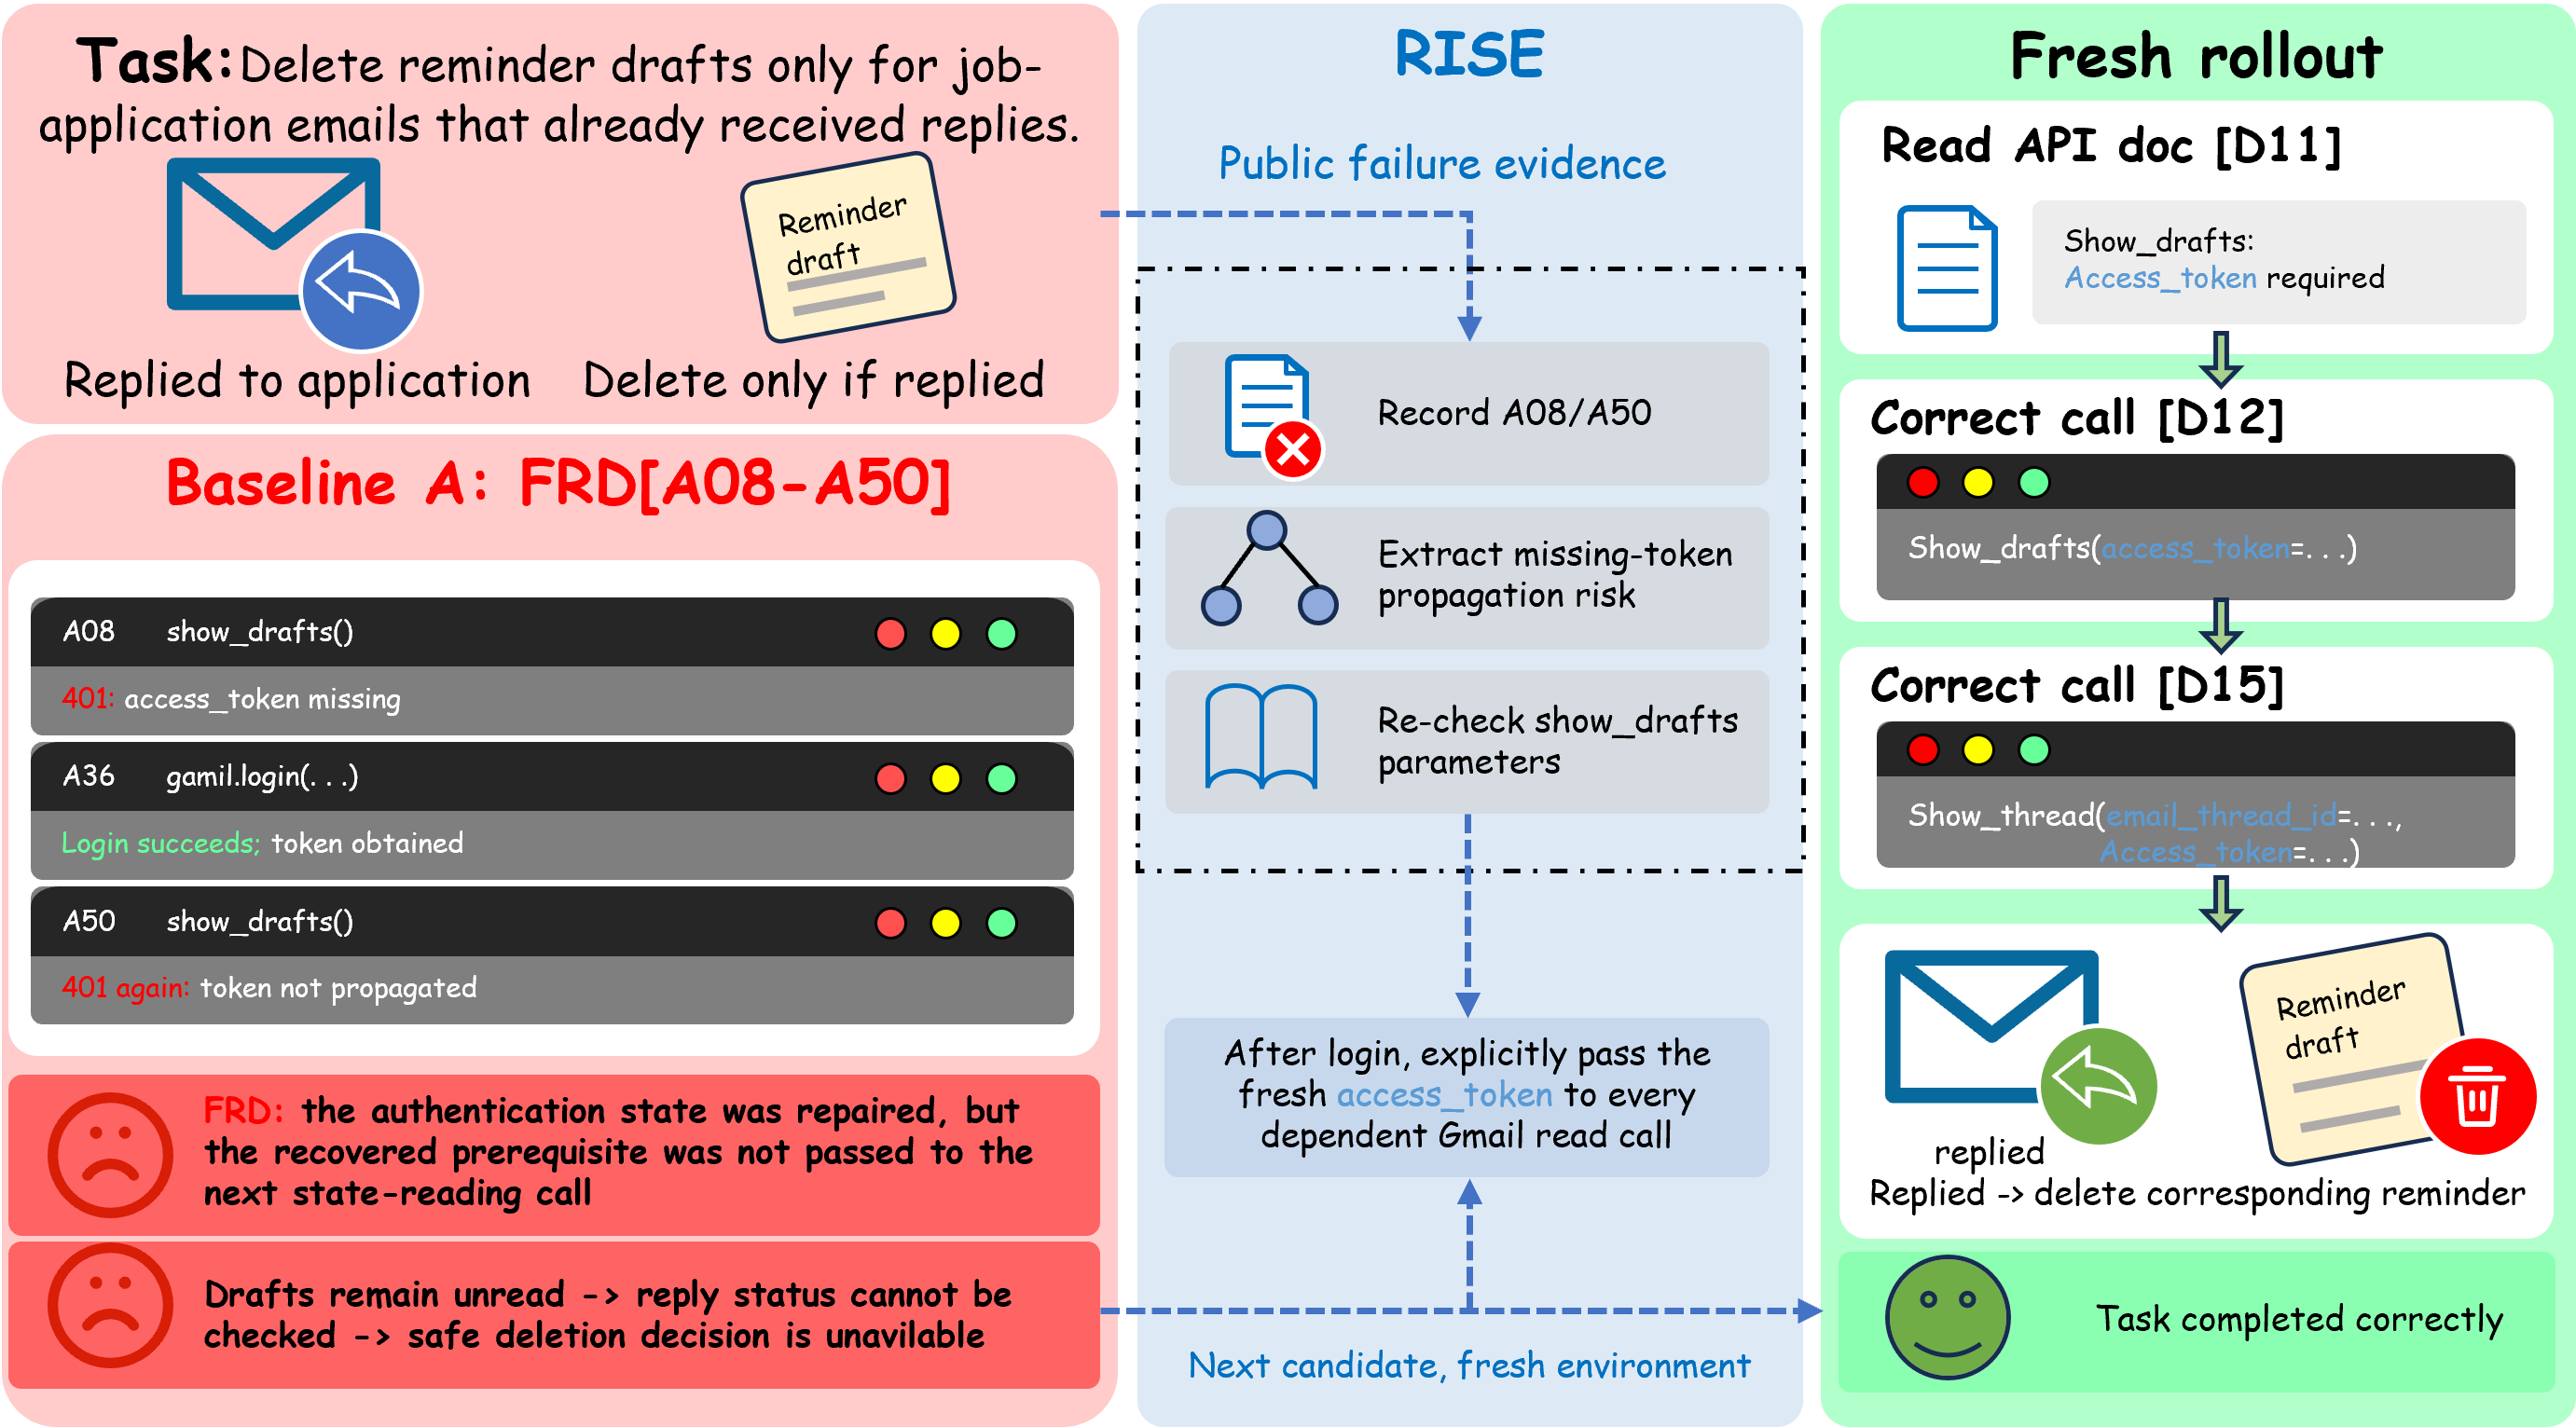
\includegraphics[width=0.55\linewidth]{figures/rise_recovery_case.png}
\caption{Guidance localizes the defect to the dependent call. The directed candidate supplies the missing credential at the retry that the baseline left unauthenticated, then completes every official check, starting from a fresh environment instead of repairing the baseline in place.}
\label{fig:rise-recovery-case}
\end{figure}

\subsection{Reduction of Failed Repair in Final Trajectories}
To measure how far \method suppresses the failure mode it targets, we compute both the adjudicated label and the public signal in the trajectories each method finally returns. As shown in Figure~\ref{fig:analysis-frd-rds}, \method lowers both quantities across the three benchmarks, and the reduction in public risk is the larger of the two because the signal covers every observable risk while the label additionally requires an attributable adverse outcome. Overall, the two panels highlight that directed rollouts avoid repeating high-risk structures and return fewer trajectories that terminate with recovery still unresolved.

\begin{figure}[t]
\centering
\begin{minipage}[t]{0.30\linewidth}\vspace{0pt}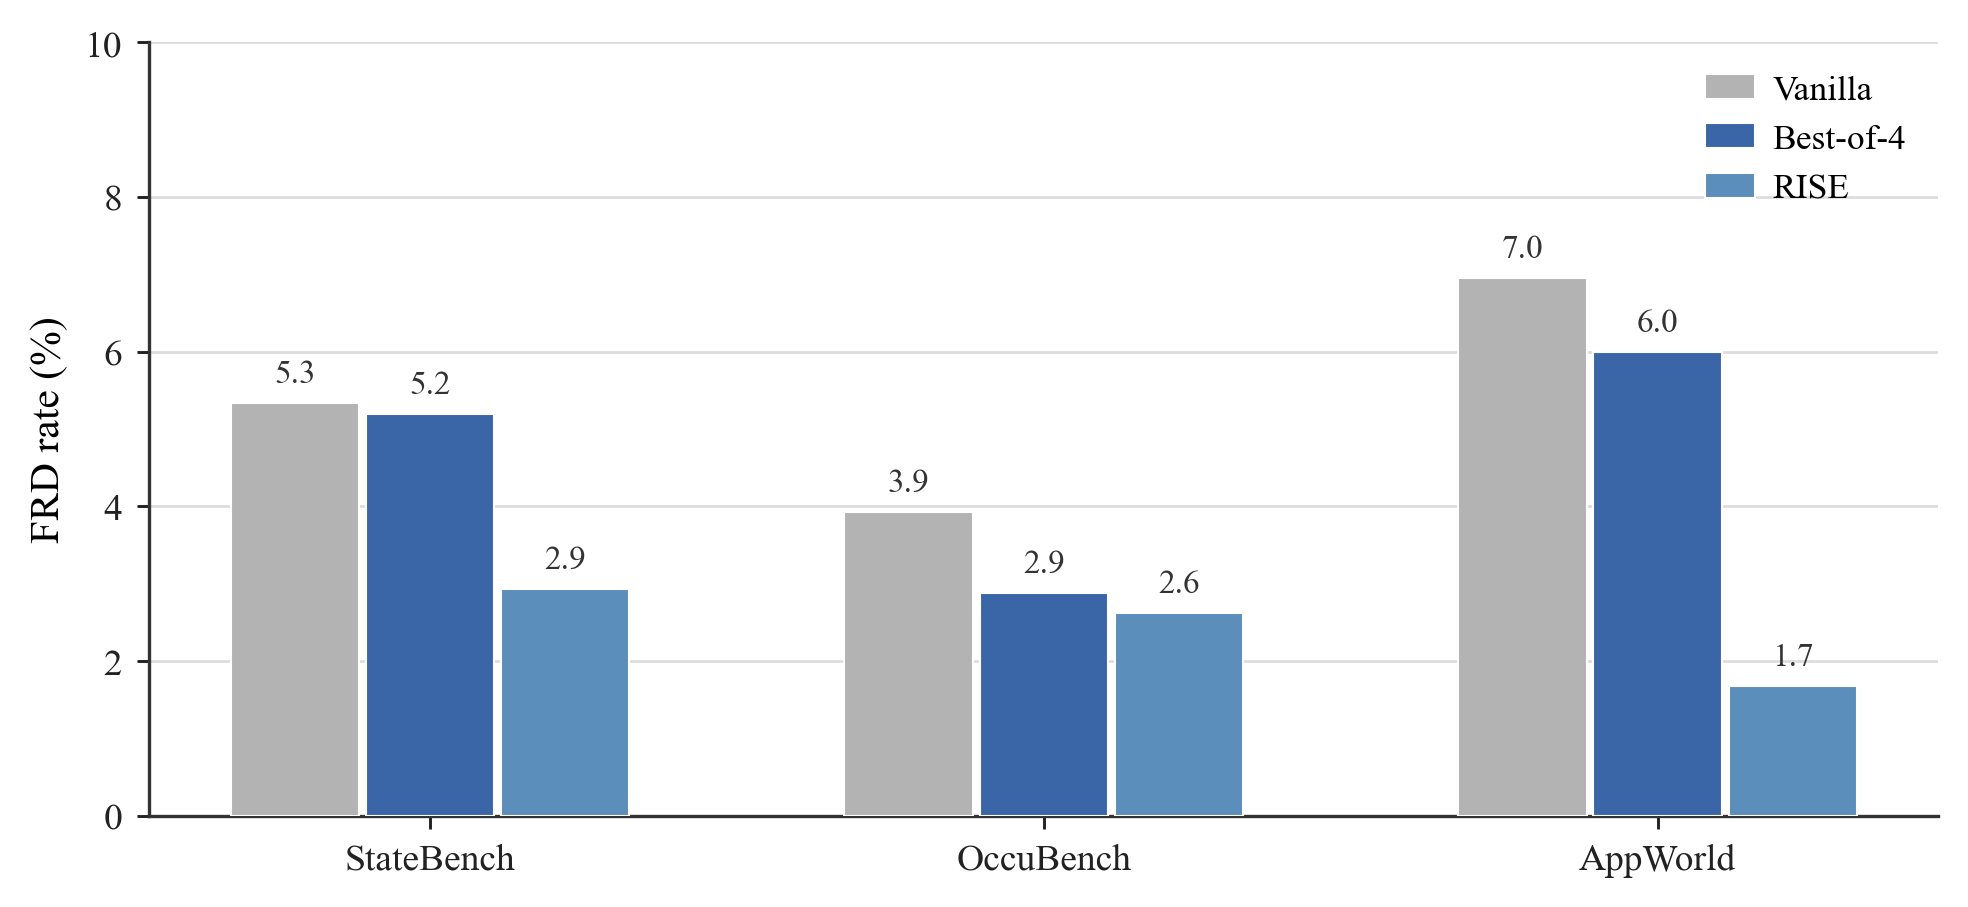
\includegraphics[width=\linewidth]{figures/rise_frd_prevalence.png}\par\vspace{2pt}\raggedright\normalfont\footnotesize (a) Adjudicated failed repair.\par\end{minipage}\hspace{0.05\linewidth}
\begin{minipage}[t]{0.30\linewidth}\vspace{0pt}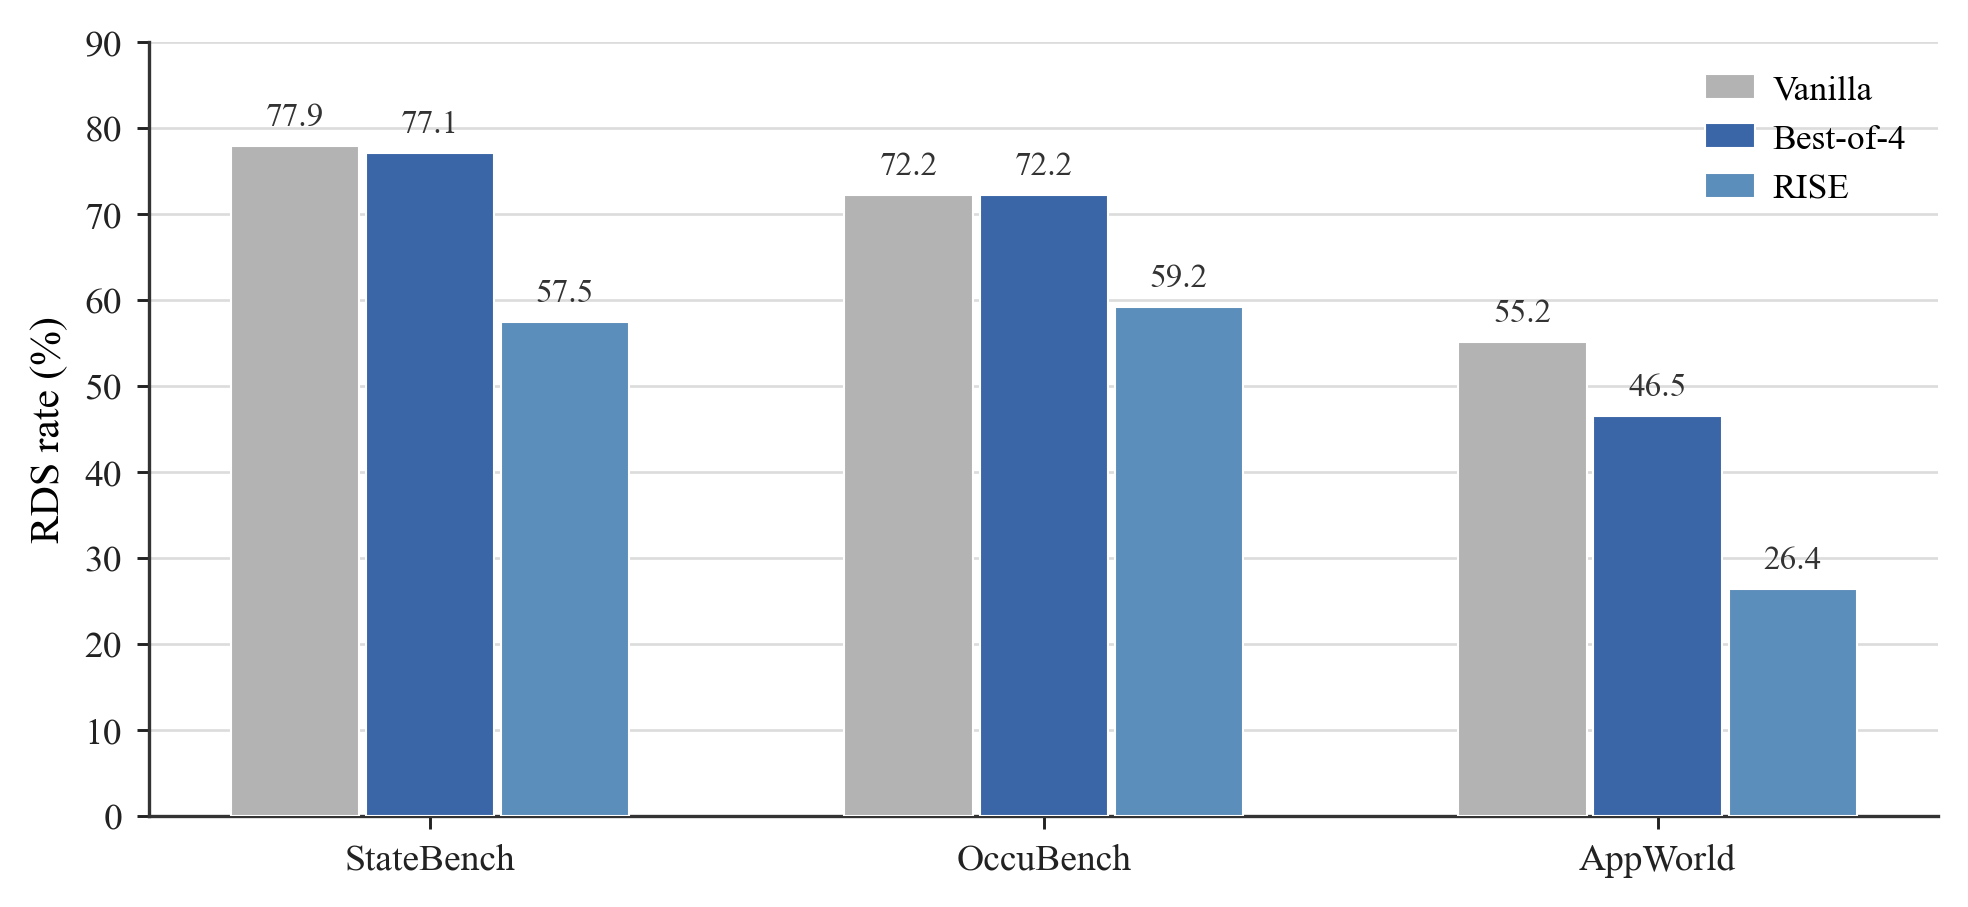
\includegraphics[width=\linewidth]{figures/rise_rds_prevalence.png}\par\vspace{2pt}\raggedright\normalfont\footnotesize (b) Public recovery risk.\par\end{minipage}
\caption{\method suppresses the failure mode it targets. Final trajectories carry less adjudicated failed repair and substantially less public recovery risk than either baseline. The gain therefore arrives through the intended mechanism.}
\label{fig:analysis-frd-rds}
\end{figure}

\subsection{Effectiveness on Risk-Positive Tasks}
To locate where the gains fall, we fix cohorts of tasks whose baseline trajectories already exhibit recovery risk and evaluate every method on that identical task set, which keeps the denominator constant across methods. As shown in Figure~\ref{fig:cohort-success}, \method improves over Vanilla on both the label-positive and signal-positive cohorts across all three benchmarks, with the widest margins on the label-positive cohort where the targeted defect is known to be present. The same procedure applied to Best-of-4 cohorts yields the same conclusion, with the strongest result on the label-positive AppWorld cohort. In particular, \method begins from its own unguided rollout instead of continuing the trajectory that defined the cohort, so these gains come from a fresh directed search. Overall, the cohort results highlight that the margin grows with the density of the defect the method was built to address.

\begin{figure}[t]
\centering
\begin{minipage}[t]{0.215\linewidth}\vspace{0pt}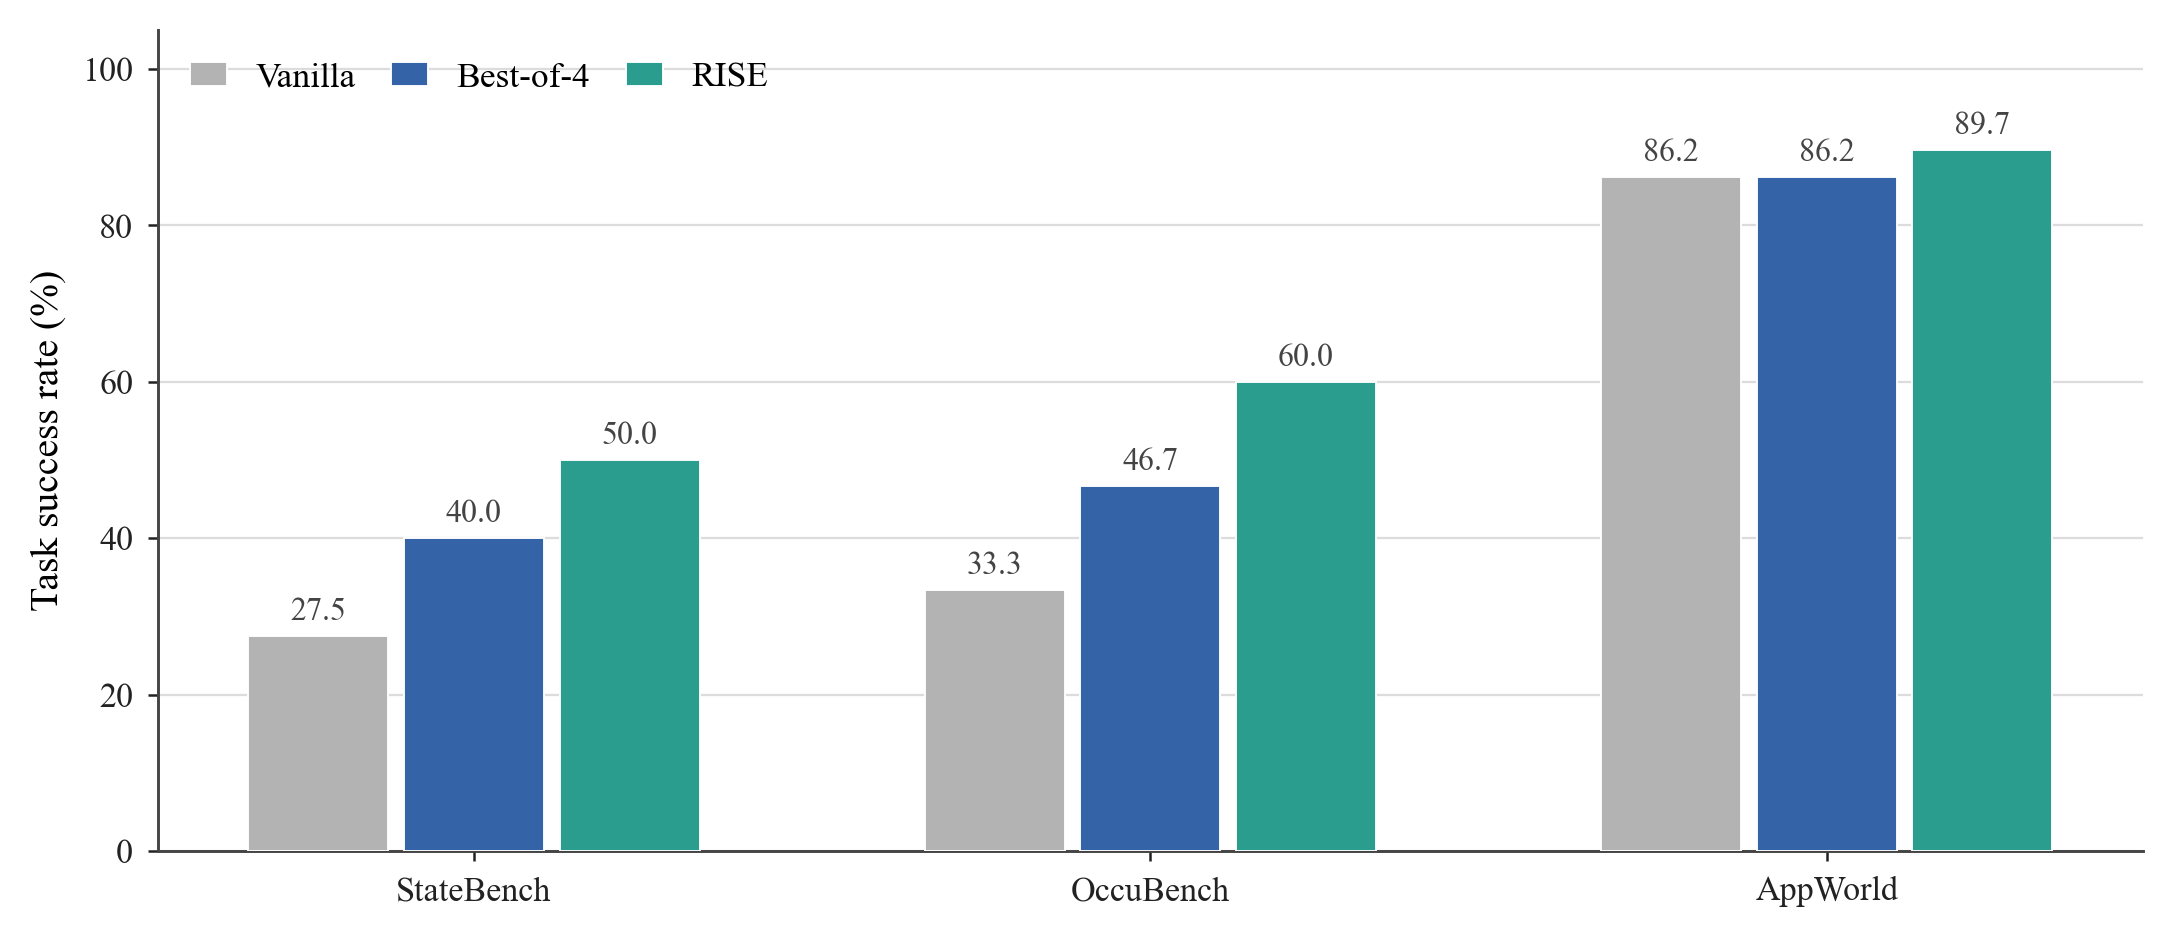
\includegraphics[width=\linewidth]{figures/cohort_frd_success.png}\par\vspace{2pt}\raggedright\normalfont\footnotesize (a) Label-positive, Vanilla.\par\end{minipage}\hfill
\begin{minipage}[t]{0.215\linewidth}\vspace{0pt}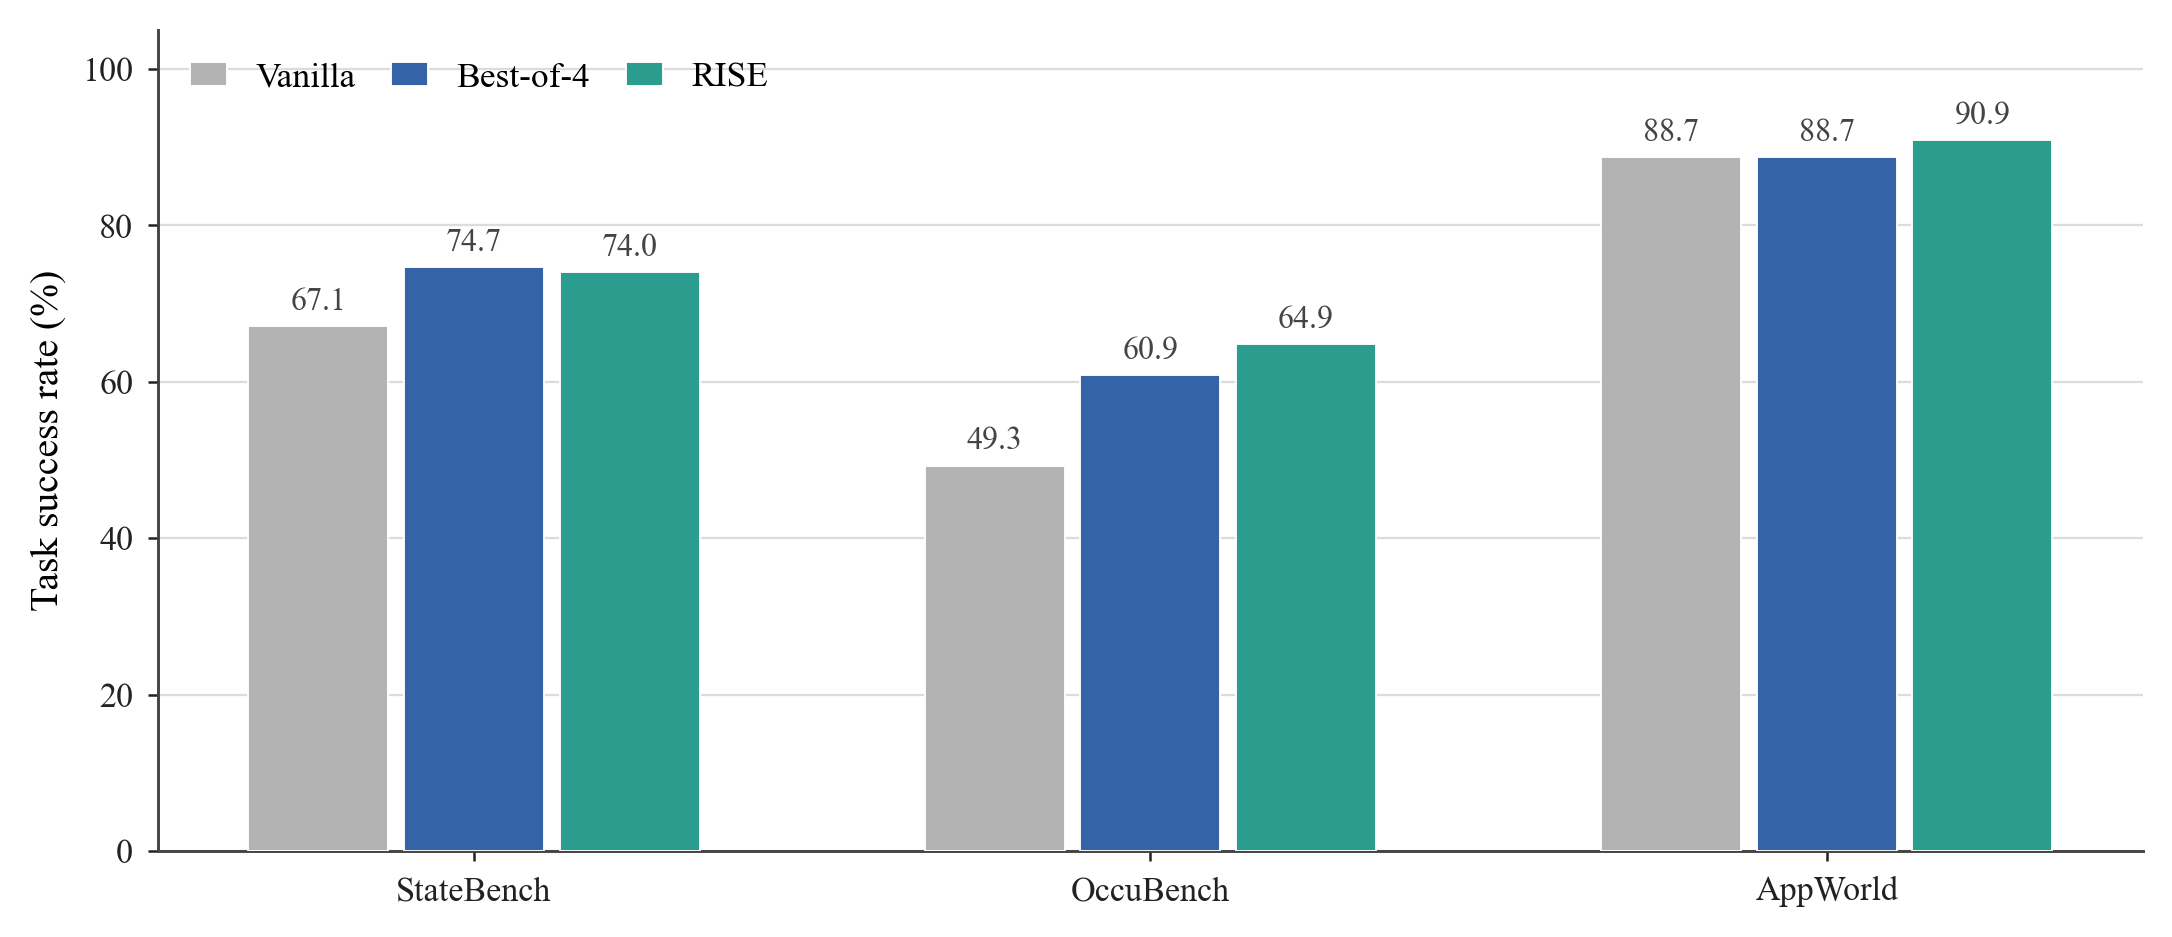
\includegraphics[width=\linewidth]{figures/cohort_rds_success.png}\par\vspace{2pt}\raggedright\normalfont\footnotesize (b) Signal-positive, Vanilla.\par\end{minipage}\hfill
\begin{minipage}[t]{0.215\linewidth}\vspace{0pt}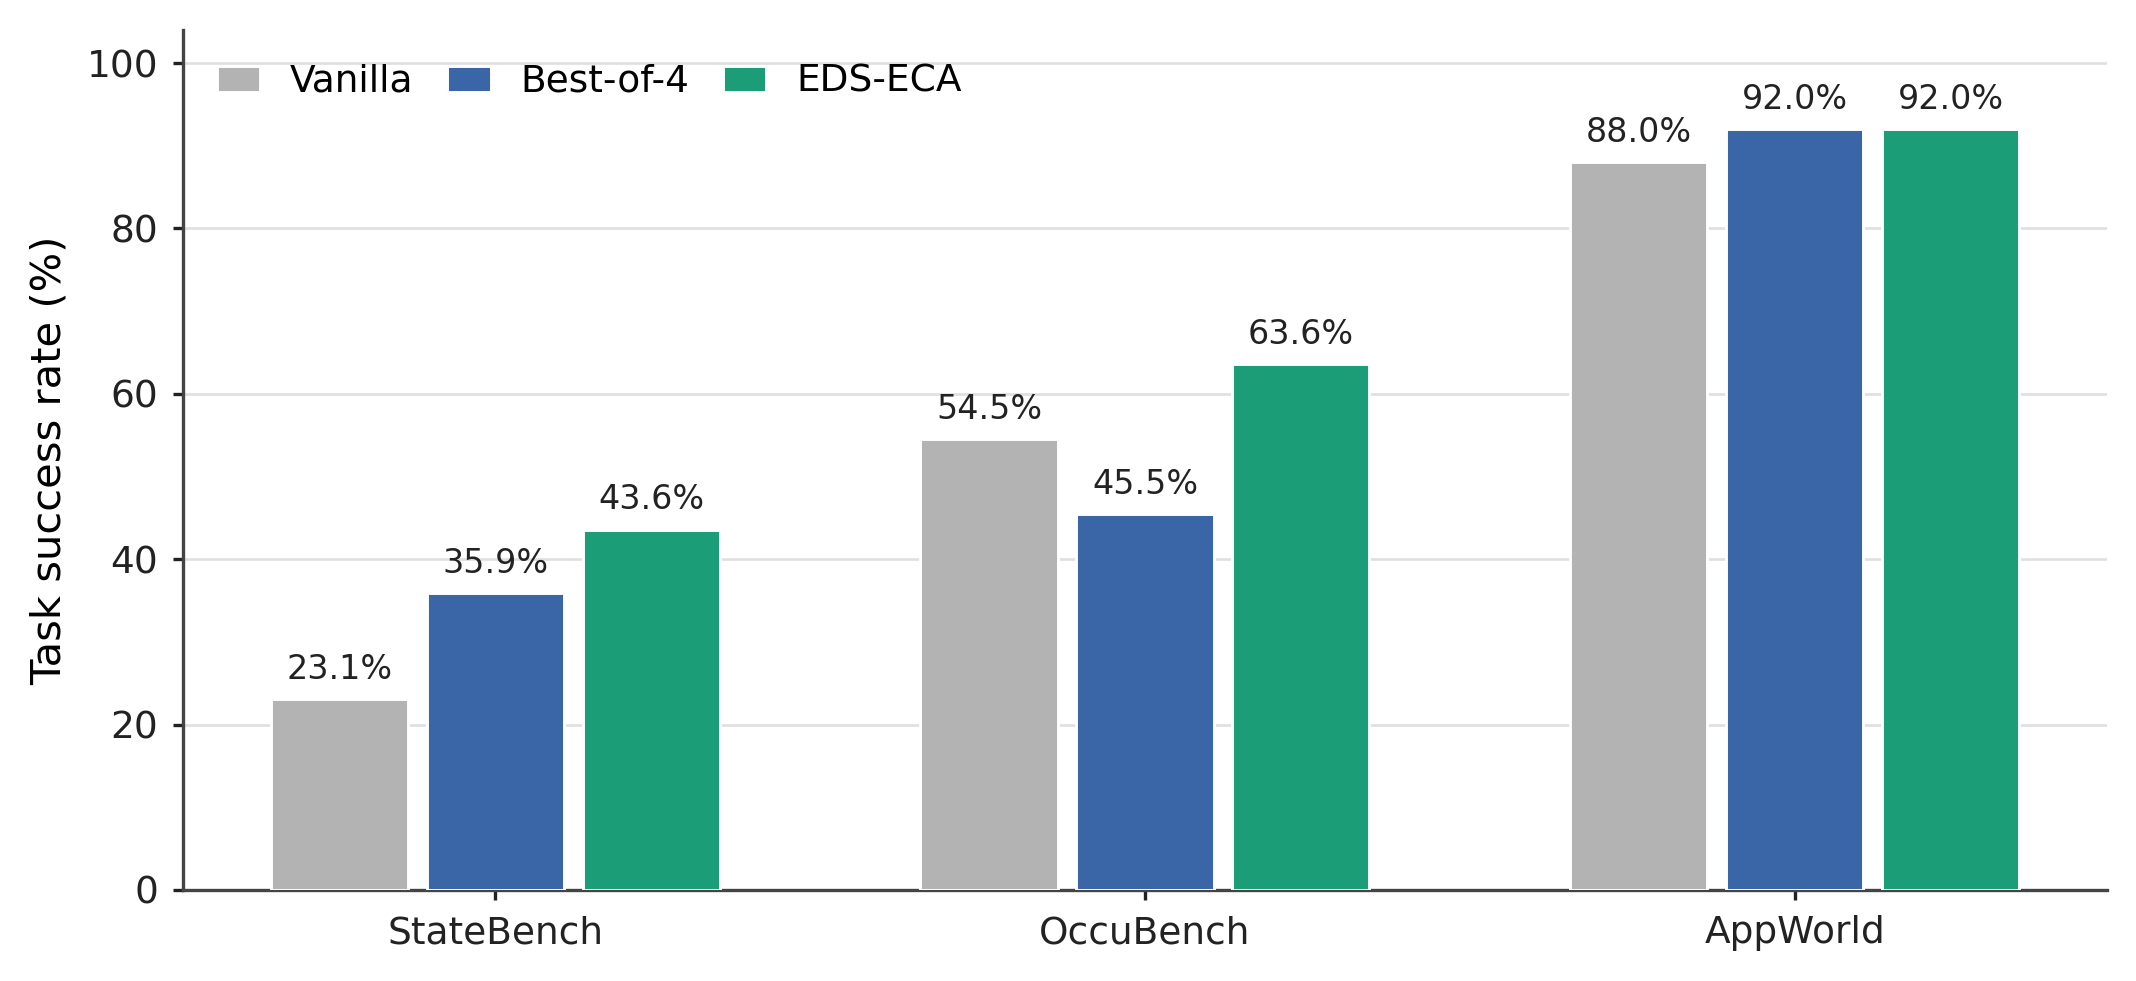
\includegraphics[width=\linewidth]{figures/best4_frd_success.png}\par\vspace{2pt}\raggedright\normalfont\footnotesize (c) Label-positive, Best-of-4.\par\end{minipage}\hfill
\begin{minipage}[t]{0.215\linewidth}\vspace{0pt}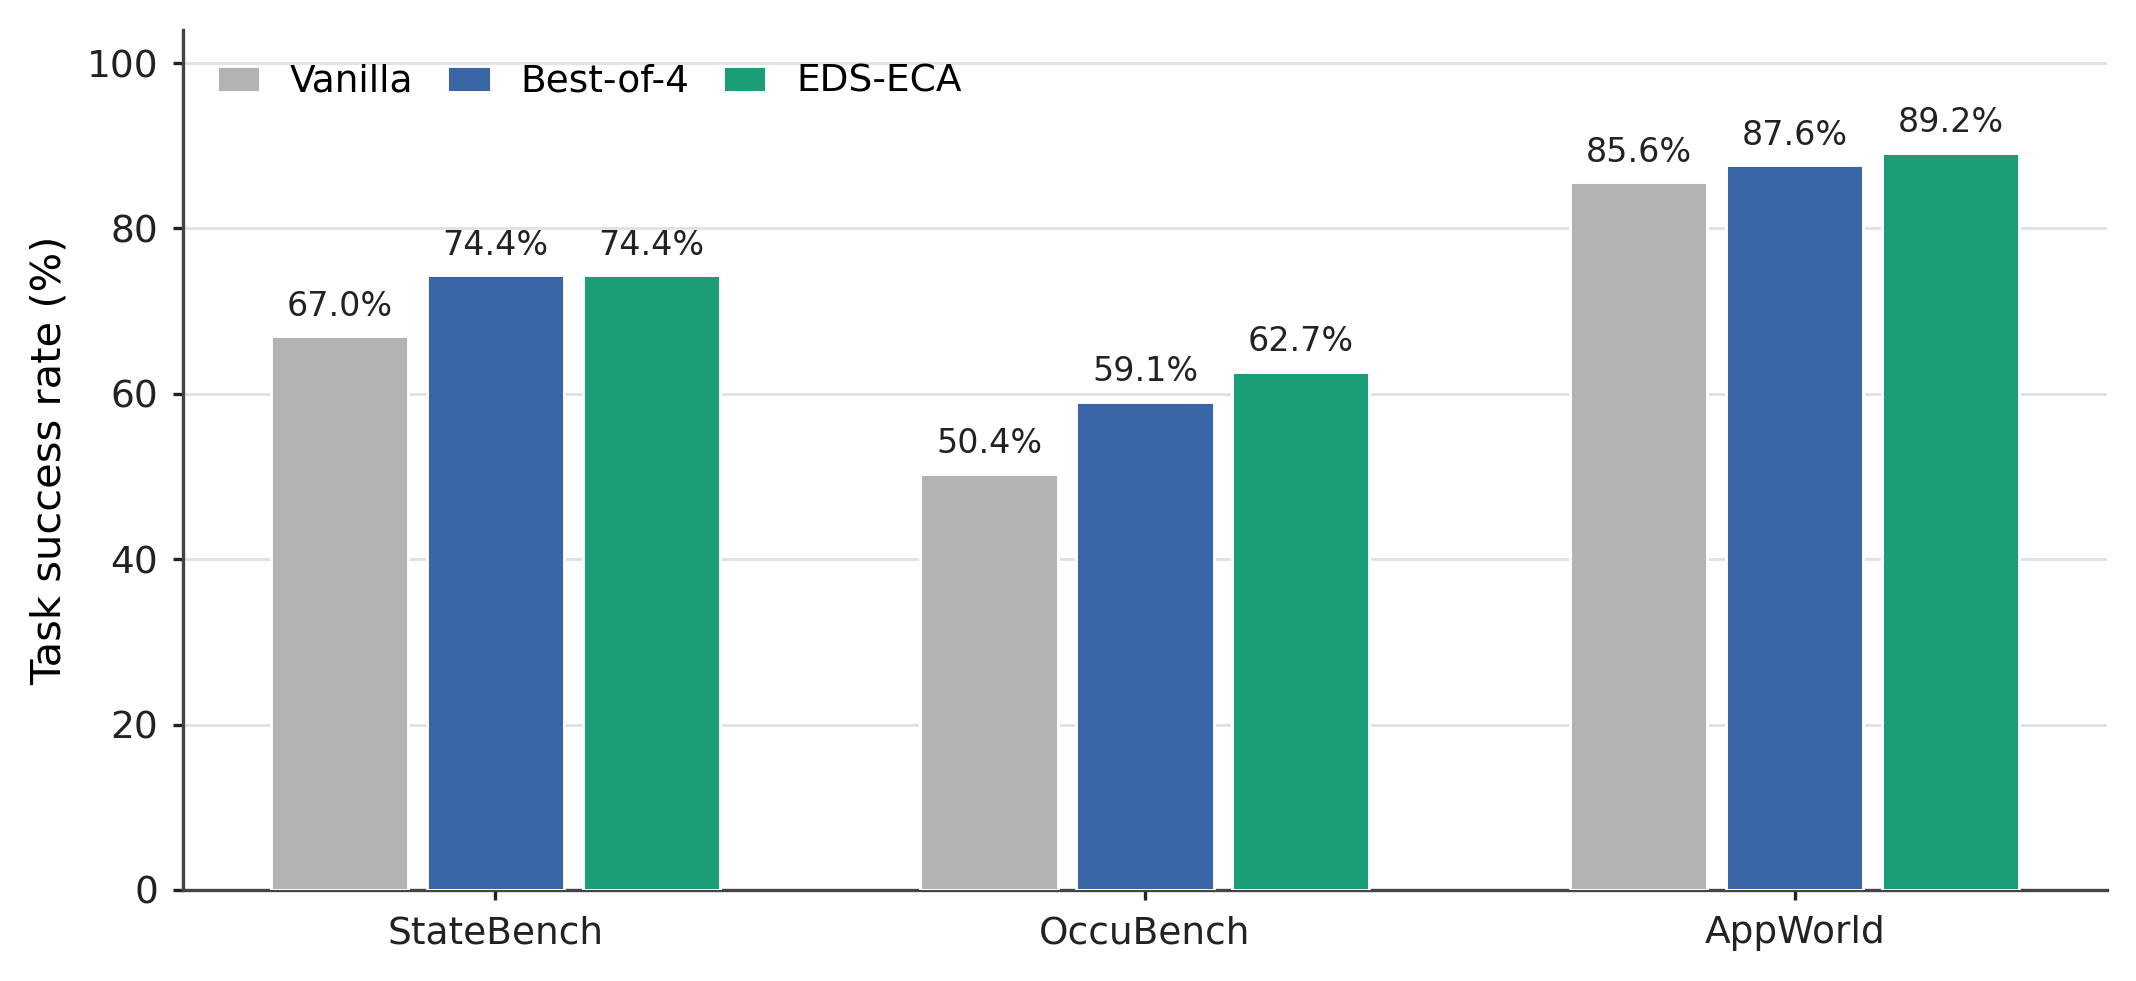
\includegraphics[width=\linewidth]{figures/best4_rds_success.png}\par\vspace{2pt}\raggedright\normalfont\footnotesize (d) Signal-positive, Best-of-4.\par\end{minipage}
\caption{Gains concentrate on tasks that carry recovery risk. On fixed cohorts with an identical denominator across methods, \method improves most where the targeted defect is known to be present, and the conclusion holds whether the cohort is drawn from Vanilla or from the stronger Best-of-4 baseline.}
\label{fig:cohort-success}
\end{figure}

\FloatBarrier
\section{Related Work}

\textbf{Tool Calling and Test-Time Selection}\quad Research on tool-using language models divides into strengthening the controller and spending additional computation at inference time. ReAct established the interleaving of reasoning, tool calls, and observations \citep{yao2023react}, and subsequent systems study design choices and reproducible comparison \citep{oagents2025}. A companion study of test-time compute evaluates parallel sampling, sequential revision, verification, and result merging, and its released configuration combines Best-of-$N$ sampling with list-wise verification \citep{oppo_tts2025}, while the verifier that ranks candidates and the benchmarks that place an agent against a mutable backend are themselves active subjects of study \citep{lightman2024verify,yao2024taubench}. Related efforts improve the controller through verified tool-use data, tutorial-guided trajectory synthesis, and world models of action-conditioned transitions \citep{mat2025,agenttrek2025,wma2025}. In essence, these approaches strengthen capability or observation quality, and their selection stage operates on finished trajectories, so comparison leaves no trace on what follows.

\textbf{Iterative Refinement at Inference Time}\quad A second line treats inference as a repeated process in which later attempts may consume the results of earlier ones. Self-consistency samples multiple reasoning paths and aggregates them \citep{wang2023selfconsistency}, Tree of Thoughts expands and evaluates intermediate states \citep{yao2023tree}, tree search over agent trajectories adds value estimates and self-reflection \citep{zhou2024lats}, and Reflexion and Self-Refine feed a verbal critique into a later attempt \citep{shinn2023reflexion,madaan2023selfrefine}. Layered proposal and aggregation frameworks extend the premise across stages \citep{moa2024}. Overall, these methods differ in what the additional computation may carry forward, with aggregation discarding the losing branches and reflection transferring unconstrained text, so neither line makes the quality of a repair a target of its own.

\textbf{Positioning}\quad In this work, we target the repair step that follows an unexpected tool result, directing a later attempt from the evidence a comparison produces. Unlike selection-based scaling, which discards every candidate it does not choose, \method converts each comparison into source-constrained structural credit, so a rejected candidate continues to shape later rollouts. Unlike reflection-based refinement, which carries free-form text, \method restricts what may transfer to value-free event shapes, which keeps guidance usable in a fresh environment and prevents stale identifiers from being replayed.

\section{Conclusion}
We identify failed repair as a distinct failure mode in tool-using language models, where a model detects an anomaly, acts on it, and still leaves the task broken. Because such a failure is adjudicable only after execution ends, we build \method on the public evidence available during a run, so that recovery risk directs each fresh rollout, an accepted trajectory preserves progress, and bilateral credit turns every comparison into a constraint on what follows.

The results support a view of test-time compute as a choice about what a budget purchases. Sampling purchases variance and pays off against failures that differ between attempts, while \method purchases information about failures that repeat, which is why its margin reaches 8.64 points over Best-of-4 on metrics that aggregate over correlated tasks. More generally, turning the evidence of an inference-time comparison into a constraint is what converts a larger budget into a better one.

\subsection*{AI Use Statement}
Generative AI tools assisted with language drafting. The authors are responsible for all claims and results reported in this paper.

\subsection*{Reproducibility Statement}
We release the core method, benchmark adapters, selector prompts, event schemas, run configurations, and evaluation scripts.

\bibliography{references}
\bibliographystyle{iclr2027_conference}

\appendix
\section{Implementation Details}
\label{app:implementation}
The event adapter supplies benchmark-specific parsing to a single search loop. StateBench exposes tool calls, arguments, and results, from which the adapter builds atomic events, transaction groups, and recovery windows. OccuBench maps action and observation traces into a compatible representation. AppWorld uses persistent Python and API interaction with explicit exceptions and structured results, where a normal business rejection is recorded as a routine outcome. The loop creates credit from a valid comparison, a no-disagreement round retains the accepted trajectory, and a returned fallback retains it as well.

\textbf{Deterministic Components}\quad The event map $f_{\mathrm{event}}$, the risk signal $f_{\mathrm{risk}}$, the frontier $f_{\mathrm{front}}$, the disagreement gate $f_{\mathrm{cmp}}$, and the credit update $f_{\mathrm{credit}}$ are deterministic functions of the public trace. Operation class is read from the API name, where a documented read prefix yields a read, a documented write prefix yields a mutation, and the session calls yield an authentication event. Result class is read from the returned payload, and a failure boundary requires an explicit exception or a status code, so a documentation lookup that merely contains the word error is not recorded as a failure. The model is invoked only by $f_{\mathrm{roll}}$ to execute a rollout and by $f_{\mathrm{sel}}$ to compare two complete candidates, which makes the guidance path reproducible for a fixed pair of traces.

\begin{algorithm}[H]
\caption{\method}
\label{alg:rise}
\small
\begin{algorithmic}[1]
\Require Task $x$, proposal schedule $\mathcal{S}$
\State $I\gets f_{\mathrm{roll}}(x,\varnothing)$; $C\gets\varnothing$; initialize $H$
\For{stage $s\in\mathcal{S}$}
  \State $V_I\gets f_{\mathrm{event}}(I)$; $\mathcal{F}\gets f_{\mathrm{front}}(V_I,C,H)$
  \State $P\gets f_{\mathrm{roll}}(x,\mathcal{F})$; $V_P\gets f_{\mathrm{event}}(P)$
  \State $D\gets f_{\mathrm{cmp}}(V_I,V_P)$
  \If{$D=0$}
    \State retain $I$ and continue
  \EndIf
  \State $q\gets f_{\mathrm{sel}}(x,V_I,V_P)$
  \If{$q$ is a fallback}
    \State retain $I$ and continue
  \EndIf
  \State $(V^s,V^r)\gets$ selected and rejected views under $q$
  \State $C\gets f_{\mathrm{credit}}(V^s,V^r,D,q,C)$
  \If{$q=\mathrm{prop}$} \State $I\gets P$ \EndIf
  \State $H\gets f_{\mathrm{hist}}(H,D,q)$
\EndFor
\State \Return $I$
\end{algorithmic}
\end{algorithm}



\section{Benchmark Details}
\label{app:benchmarks}
\textbf{StateBench} evaluates stateful conversational tool use across travel, customer support, and shopping assistance, comprising 150 test tasks. It reports PASS@1 for average completion, PASS$^5$ for completion in all five independent runs, and UX for user experience rated from one to five. The five runs use five generation, selector, and judge seeds, and every method is evaluated under the same seed set.

\textbf{AppWorld} \citep{trivedi2024appworld} evaluates persistent Python and API interaction across applications, comprising 168 tasks over 56 scenarios in Test-Normal and 417 tasks over 139 scenarios in Test-Challenge. It reports task goal completion and scenario goal completion, where a scenario passes only if every task in its group passes.

\textbf{OccuBench} evaluates tool calling in professional settings spanning ten occupational domains, comprising 382 tasks whose tool responses and fault conditions are supplied by a language world model. It reports PASS@1 over its evaluation instances.

\textbf{DeepPlanning Travel} evaluates travel planning under commonsense and personalized constraints, comprising 240 cases split evenly between Chinese and English. It reports Delivery, Commonsense, Personalized, and Composite scores in each language.

\section{Adjudication Protocol}
\label{app:adjudication}
Every quantity reported in Section~\ref{sec:analysis} depends on how a recovery episode is judged, so we state the procedure before the results that rely on it. An episode enters adjudication only when the public trace contains a concrete recovery entry, meaning an explicit diagnosis, a retry, or a corrective call that follows an anomaly. The adjudicator then answers three questions in order. It first determines whether a recovery need exists, which may originate from a failed call, an inconsistent state, or a user-reported problem. It next determines whether the trajectory attempts a recovery decision at that point. It finally determines whether an adverse outcome follows and whether that outcome is attributable to the decision under review.

An episode is labelled positive when all three answers are affirmative and the trace supports the attribution, and the remaining episodes are recorded under their observed outcome. We record the recovery outcome separately from whether the benchmark task ultimately passed, since a later successful repair does not retract an earlier failed one.

\textbf{Agreement}\quad Each episode is judged independently by multiple annotators under the instruction above, and disagreements are resolved by discussion before a label is recorded. The annotation interface and the full instruction accompany the released materials.

\section{Credit Construction}
\label{app:credit}
\textbf{Preserve Eligibility}\quad Let $E_s$ and $E_r$ be the selected and rejected event sets and let $\mathcal{B}$ denote rejected, failed, and error results. Before deterministic sorting and truncation, preserve eligibility is
\begin{equation}
\begin{split}
\mathcal{P}(E_s,E_r)=\{e\in E_s:\;&\mathrm{result}(e)\notin\mathcal{B}\ \land\\
&[\mathrm{shape}(e)\notin\mathrm{Shape}(E_r)\ \lor\ \mathrm{class}(e)\in\{\mathrm{mutation},\mathrm{verification}\}]\}.
\end{split}
\label{eq:preserve}
\end{equation}
A shape records operation, event class, tool, entity field names, argument keys, result class, and interaction type, and excludes literal argument values. Avoid eligibility uses rejected-side risk identifiers, failure results, and structural differences under the same projection. Eligibility ranks structures by the scrutiny the next rollout should give them.

\end{document}
